%%%%%%%%%%%%%%%%%%%%%%%%%%%%%%%%%%%%%%%%%%%%%%%%%%%%%%%%%%%%%%%%%%%%%
% LaTeX Template: Project Titlepage Modified (v 0.1) by rcx
%
% Original Source: http://www.howtotex.com
% Date: February 2014
% 
% This is a title page template which be used for articles & reports.
% 
% This is the modified version of the original Latex template from
% aforementioned website.
% 
%%%%%%%%%%%%%%%%%%%%%%%%%%%%%%%%%%%%%%%%%%%%%%%%%%%%%%%%%%%%%%%%%%%%%%

\documentclass[12pt]{report}
\usepackage[a4paper]{geometry}
\usepackage[myheadings]{fullpage}
\usepackage{fancyhdr}
\usepackage{lastpage}
\usepackage{graphicx, wrapfig,setspace, booktabs}
\usepackage[T1]{fontenc}
\usepackage[font=small, labelfont=bf]{caption}
\usepackage{fourier}
\usepackage[protrusion=true, expansion=true]{microtype}
\usepackage[english]{babel}
\usepackage{sectsty}
\usepackage{lipsum}
\usepackage[hyphens]{url}
%\usepackage{subfig}
\usepackage{hyperref}
\usepackage{alphalph}
\usepackage[utf8]{inputenc}
\usepackage{multicol}
\usepackage{amsmath}
\usepackage{subfigure}
\renewcommand*{\thesubfigure}{%
\alphalph{\value{subfigure}}%
}%


\newcommand{\HRule}[1]{\rule{\linewidth}{#1}}
\onehalfspacing
\setcounter{tocdepth}{5}
\setcounter{secnumdepth}{5}
\usepackage{float}

\usepackage[backend=bibtex,style=chem-acs,biblabel=dot]{biblatex}
\addbibresource{references.bib}

%-------------------------------------------------------------------------------
% HEADER & FOOTER
%-------------------------------------------------------------------------------
\pagestyle{fancy}
\fancyhf{}
\setlength\headheight{15pt}
\fancyhead[L]{CS7015: PA4}
\fancyhead[R]{Deep Learning}
\fancyfoot[R]{Page \thepage\ of \pageref{LastPage}}
%-------------------------------------------------------------------------------
% TITLE PAGE
%-------------------------------------------------------------------------------

\begin{document}

\title{ \normalsize \textsc{CS7015 : Deep Learning}
		\\ [2.0cm]
		\HRule{0.5pt} \\
		\LARGE \textbf{\uppercase{Programming Assignment 5}}\\
        \large{- RBM -}
		\HRule{2pt} \\ [0.5cm]
		\normalsize \today \vspace*{5\baselineskip}}

\date{}

\author{
		Student ID:  \\ 
		Namida M - EE15B123 \\
		Ganga Meghanath - EE15B025
		}

\renewcommand\thesection{\arabic{section}}
\maketitle
\tableofcontents
\newpage

%-------------------------------------------------------------------------------
% Section title formatting
\sectionfont{\scshape}
%-------------------------------------------------------------------------------

%-------------------------------------------------------------------------------
% BODY
%-------------------------------------------------------------------------------

\section{Introduction}
RBMs can be used to learn hidden representations (h) from the raw features (V ). The objective of the assignment is to train RBMs using the Contrastive Divergence (CD) algorithm. The training data used is Fashion MNIST. The 784 dimensional (V) dataset is thresholded into binary data (using a threshold of 127) to learn a n-dimensional hidden representation (h).
%-------------------------------------------------------------------------------
%DATA ANALYSIS
%-------------------------------------------------------------------------------

\section{t-SNE Plots}

\subsection{lr = 1e-3, n = 256}
The t-SNE plots for train and test data has been depicted below :

\begin{table}[H]
  \centering
  \begin{tabular}{ | c | c | c | c || c |}
    \hline
    \textbf{lr} & \textbf{n} & \textbf{k} & \textbf{Train t-SNE} & \textbf{Test t-SNE}  \\ \hline
    1e-3 & 256 & 1 &
    \begin{minipage}{.3\textwidth}
      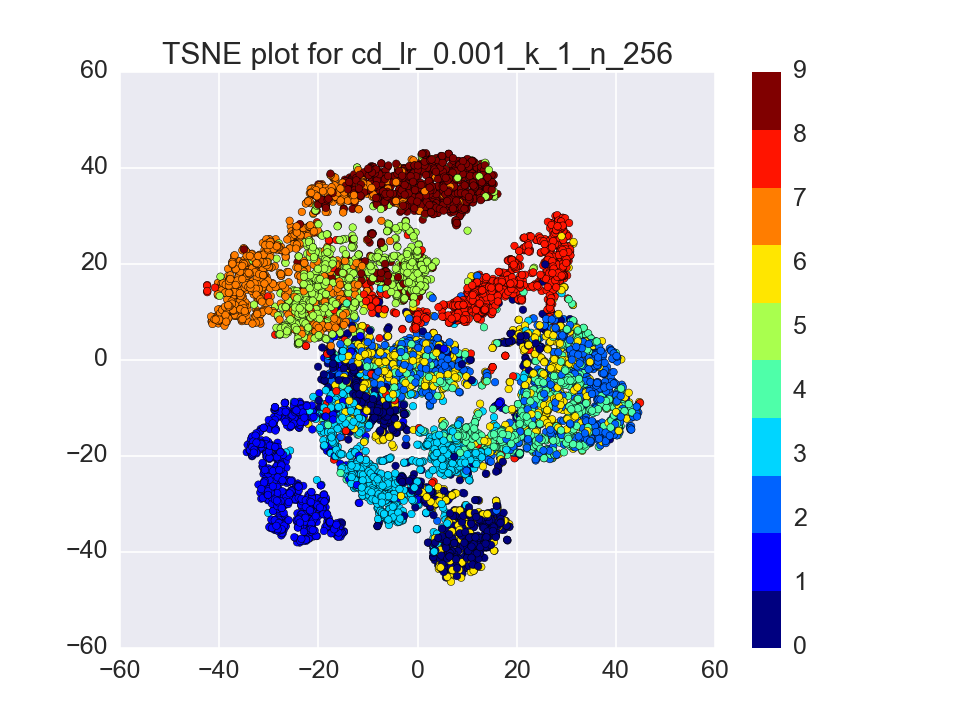
\includegraphics[scale=0.25]{cd_lr_0_001_k_1_n_256.png}
    \end{minipage} &
    \begin{minipage}{.3\textwidth}
      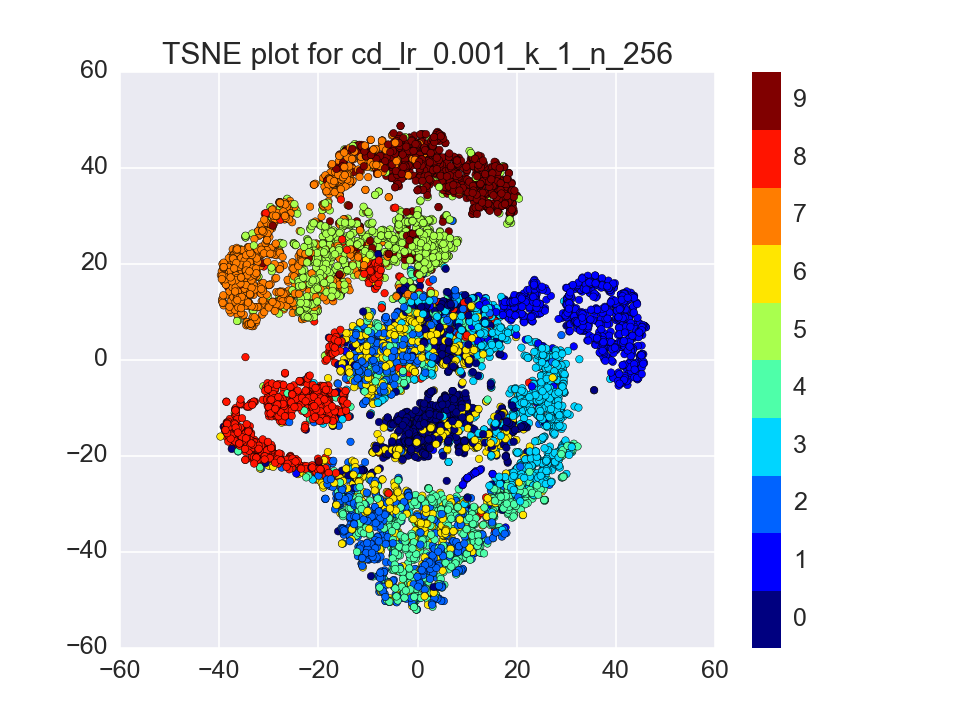
\includegraphics[scale=0.25]{test_cd_lr_0_001_k_1_n_256.png}
    \end{minipage}
    \\ \hline
    1e-3 & 256 & 2 &
    \begin{minipage}{.3\textwidth}
      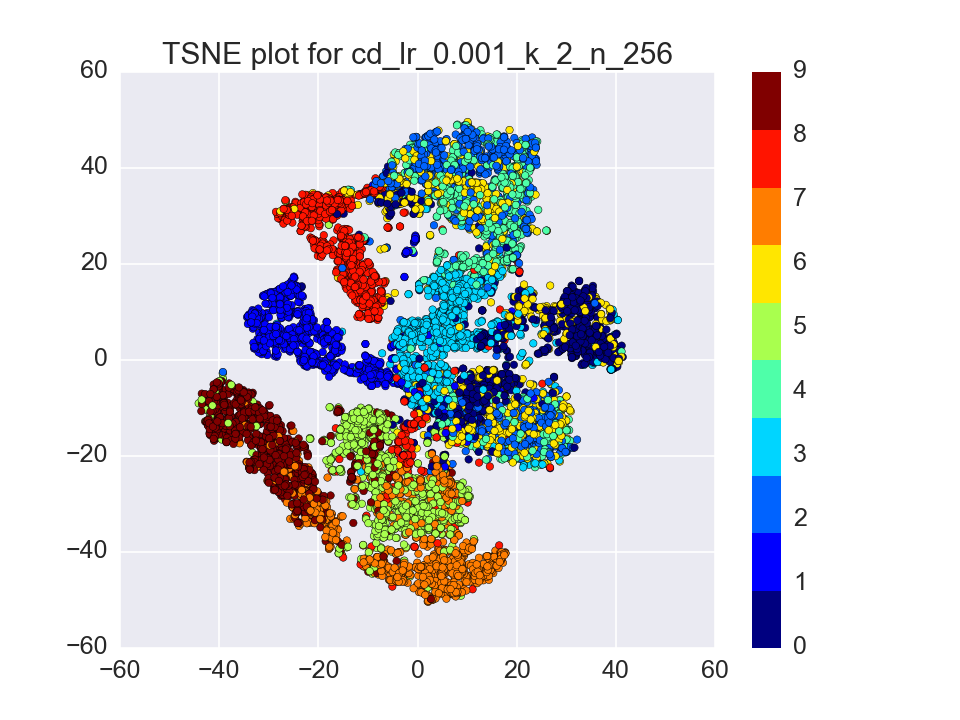
\includegraphics[scale=0.25]{cd_lr_0_001_k_2_n_256.png}
      %\includegraphics[width=\linewidth, height=60mm]{tiger}
    \end{minipage} &
    \begin{minipage}{.3\textwidth}
      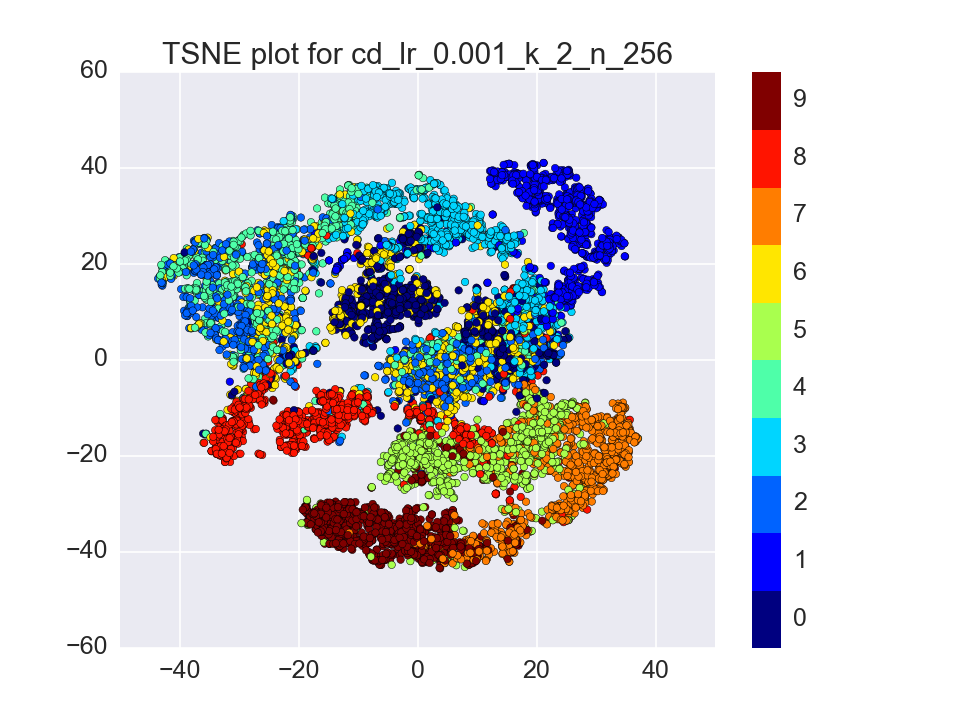
\includegraphics[scale=0.25]{test_cd_lr_0_001_k_2_n_256.png}
      %\includegraphics[width=\linewidth, height=60mm]{tiger}
    \end{minipage}
    \\ \hline
    1e-3 & 256 & 4 &
    \begin{minipage}{.3\textwidth}
      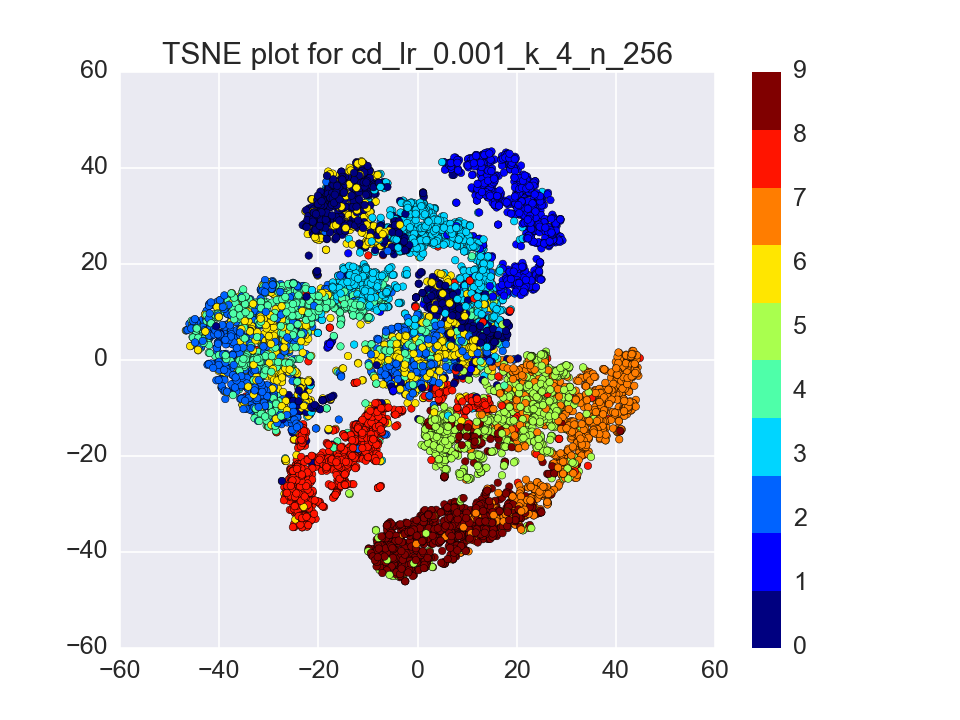
\includegraphics[scale=0.25]{cd_lr_0_001_k_4_n_256.png}
      %\includegraphics[width=\linewidth, height=60mm]{tiger}
    \end{minipage} &
    \begin{minipage}{.3\textwidth}
      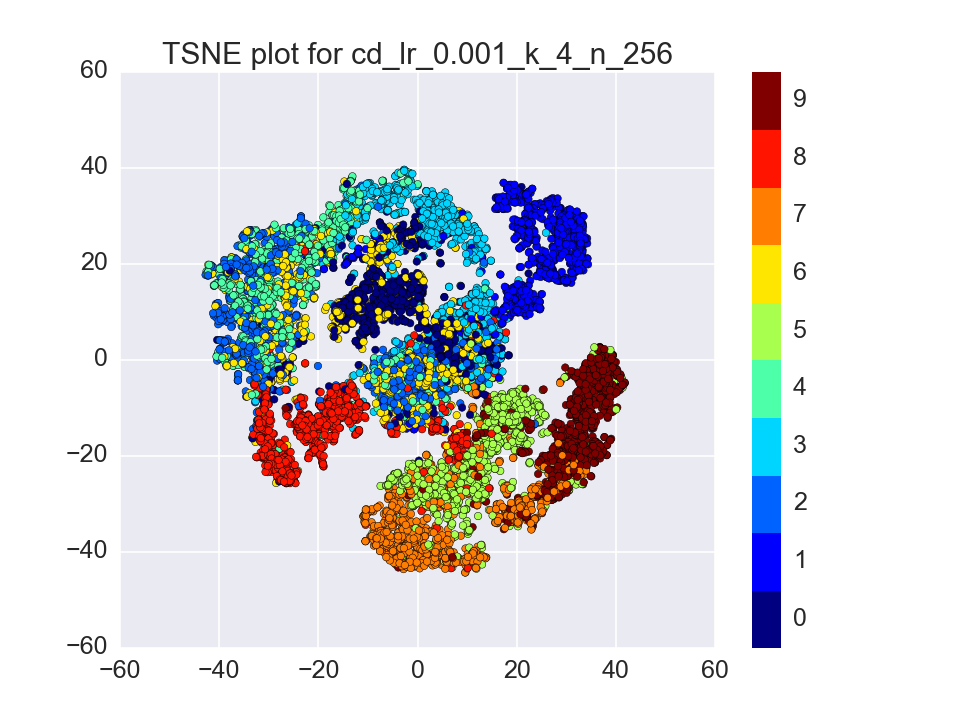
\includegraphics[scale=0.25]{test_cd_lr_0_001_k_4_n_256.png}
      %\includegraphics[width=\linewidth, height=60mm]{tiger}
    \end{minipage}
        \\ \hline
  \end{tabular}
\end{table}

\begin{table}[H]
  \centering
  \begin{tabular}{ | c | c | c | c || c |}
    \hline
    \textbf{lr} & \textbf{n} & \textbf{k} & \textbf{Train t-SNE} & \textbf{Test t-SNE}\\ \hline
    1e-3 & 256 & 8 &
    \begin{minipage}{.3\textwidth}
      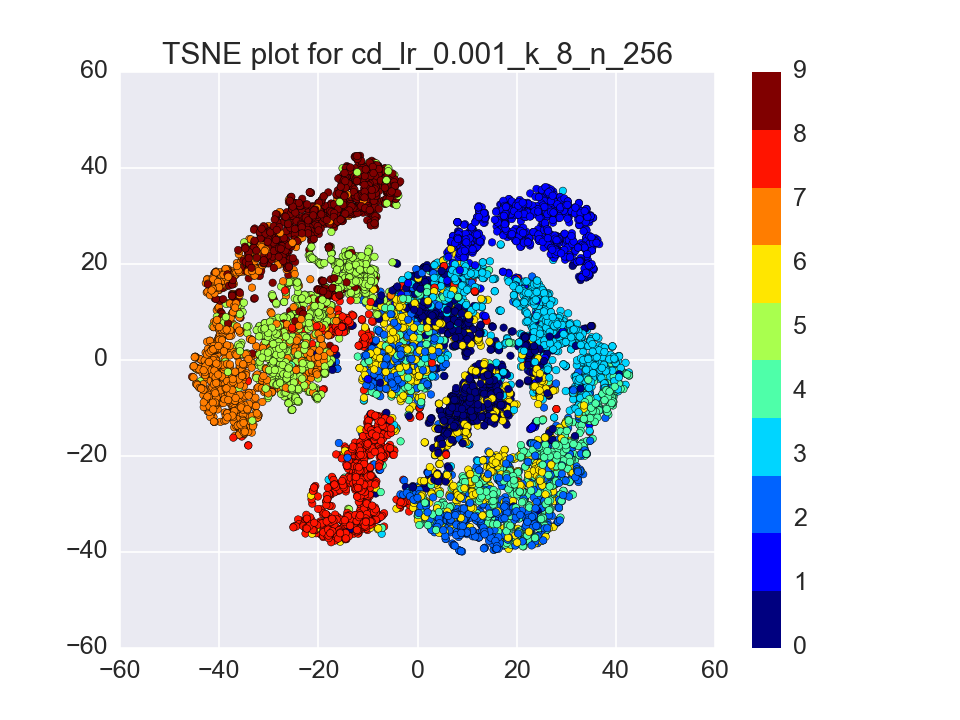
\includegraphics[scale=0.25]{cd_lr_0_001_k_8_n_256.png}
      %\includegraphics[width=\linewidth, height=60mm]{tiger}
    \end{minipage} &
    \begin{minipage}{.3\textwidth}
      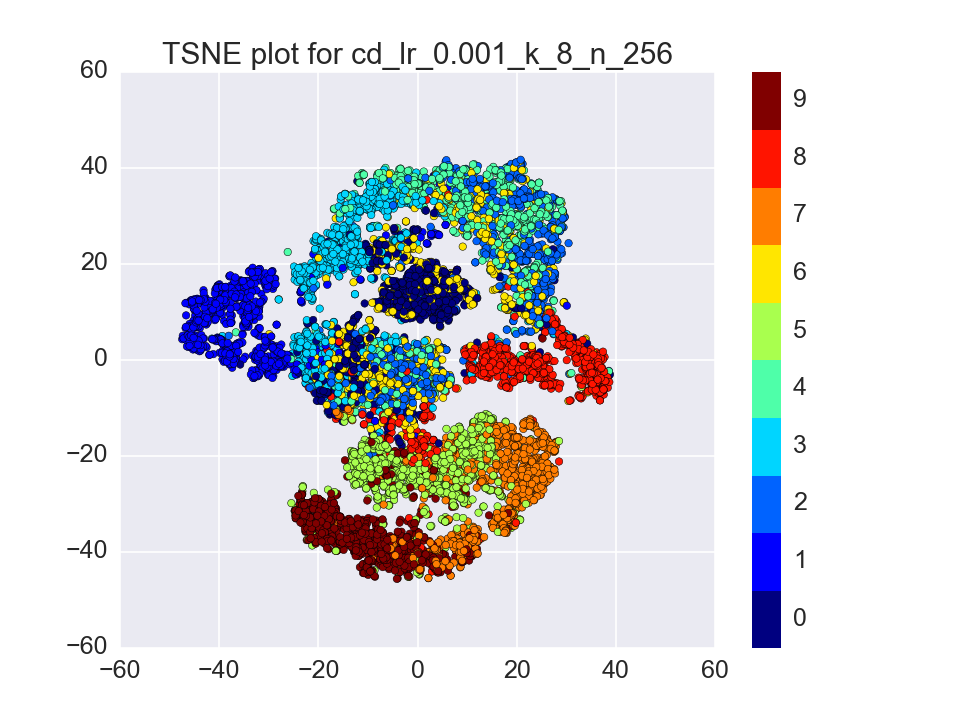
\includegraphics[scale=0.25]{test_cd_lr_0_001_k_8_n_256.png}
      %\includegraphics[width=\linewidth, height=60mm]{tiger}
    \end{minipage}
        \\ \hline
    1e-3 & 256 & 16 &
    \begin{minipage}{.3\textwidth}
      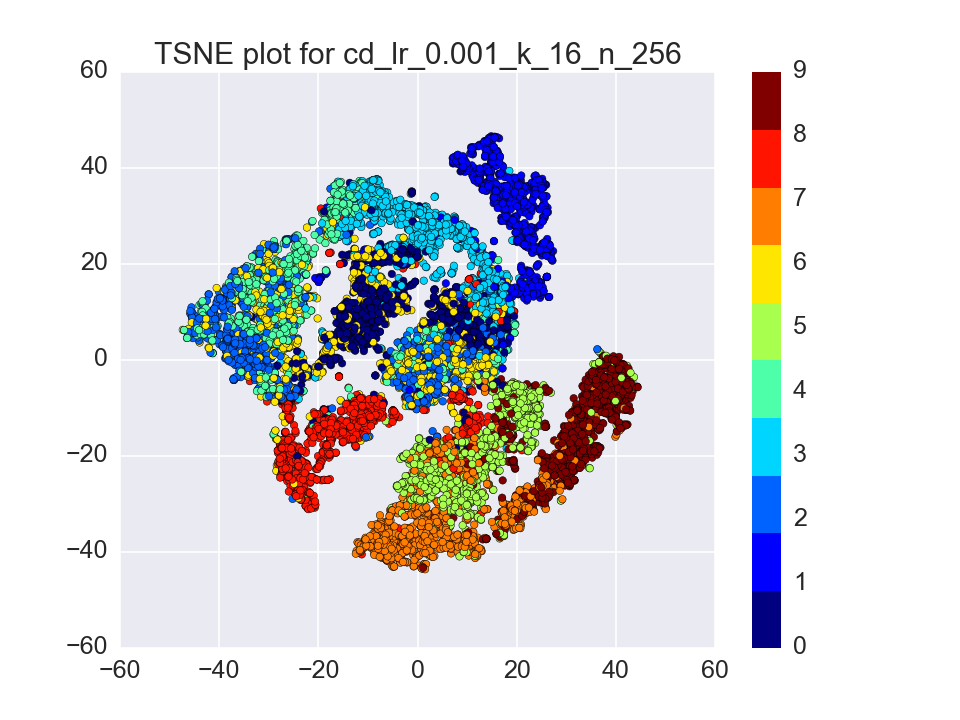
\includegraphics[scale=0.25]{cd_lr_0_001_k_16_n_256.png}
      %\includegraphics[width=\linewidth, height=60mm]{tiger}
    \end{minipage} &
    \begin{minipage}{.3\textwidth}
      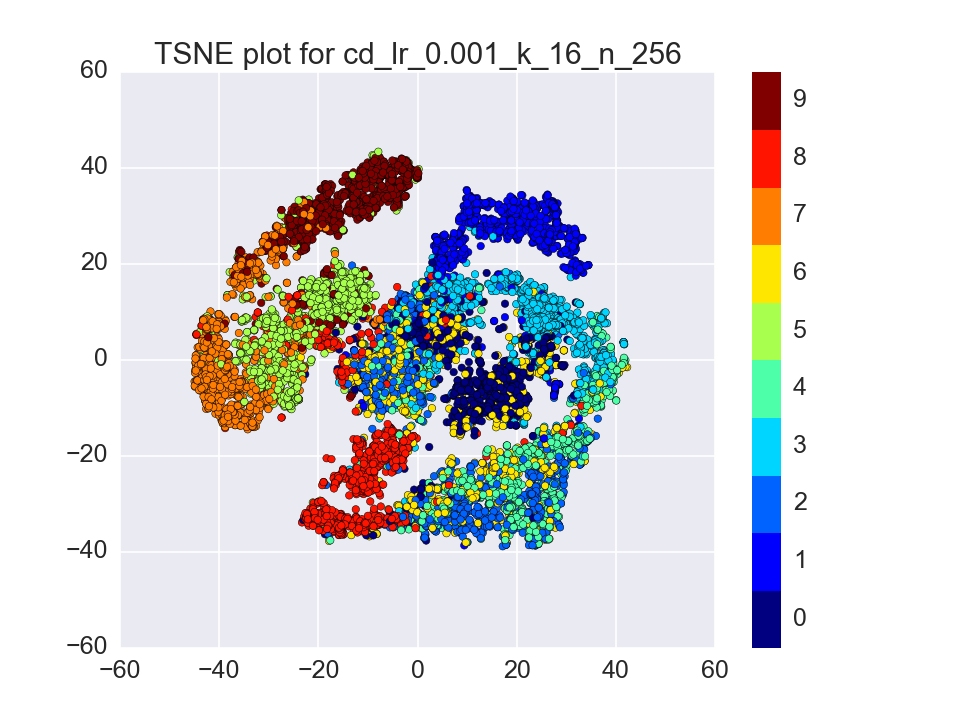
\includegraphics[scale=0.25]{test_cd_lr_0_001_k_16_n_256.png}
      %\includegraphics[width=\linewidth, height=60mm]{tiger}
    \end{minipage}
        \\ \hline
    1e-3 & 256 & 32 &
    \begin{minipage}{.3\textwidth}
      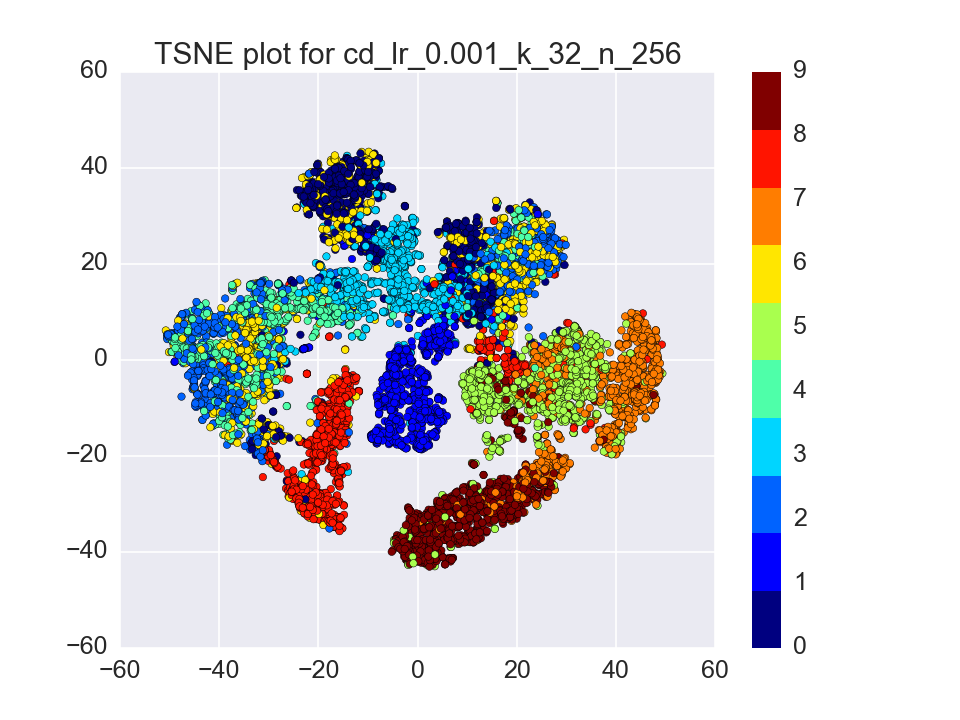
\includegraphics[scale=0.25]{cd_lr_0_001_k_32_n_256.png}
      %\includegraphics[width=\linewidth, height=60mm]{tiger}
    \end{minipage} &
    \begin{minipage}{.3\textwidth}
      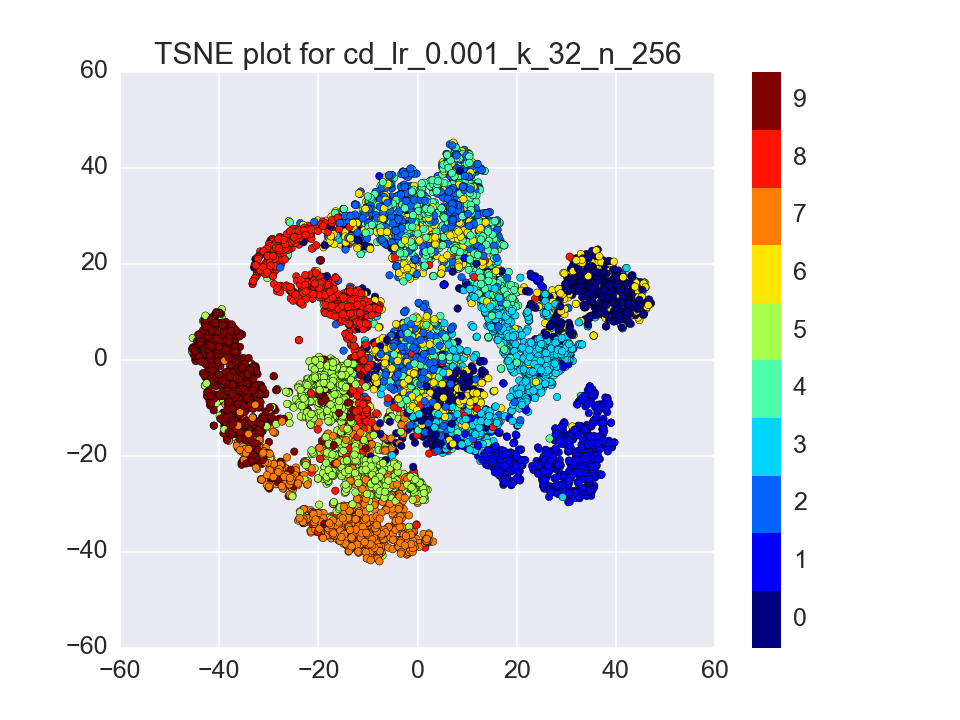
\includegraphics[scale=0.25]{test_cd_lr_0_001_k_32_n_256.png}
      %\includegraphics[width=\linewidth, height=60mm]{tiger}
    \end{minipage}
   \\ \hline
  \end{tabular}
\end{table}


\subsection{lr = 1e-3, n = 128}
\begin{table}[H]
  \centering
  \begin{tabular}{ | c | c | c | c || c |}
    \hline
    \textbf{lr} & \textbf{n} & \textbf{k} & \textbf{Train t-SNE} & \textbf{Test t-SNE}\\ \hline
    1e-3 & 128 & 1 &
    \begin{minipage}{.3\textwidth}
      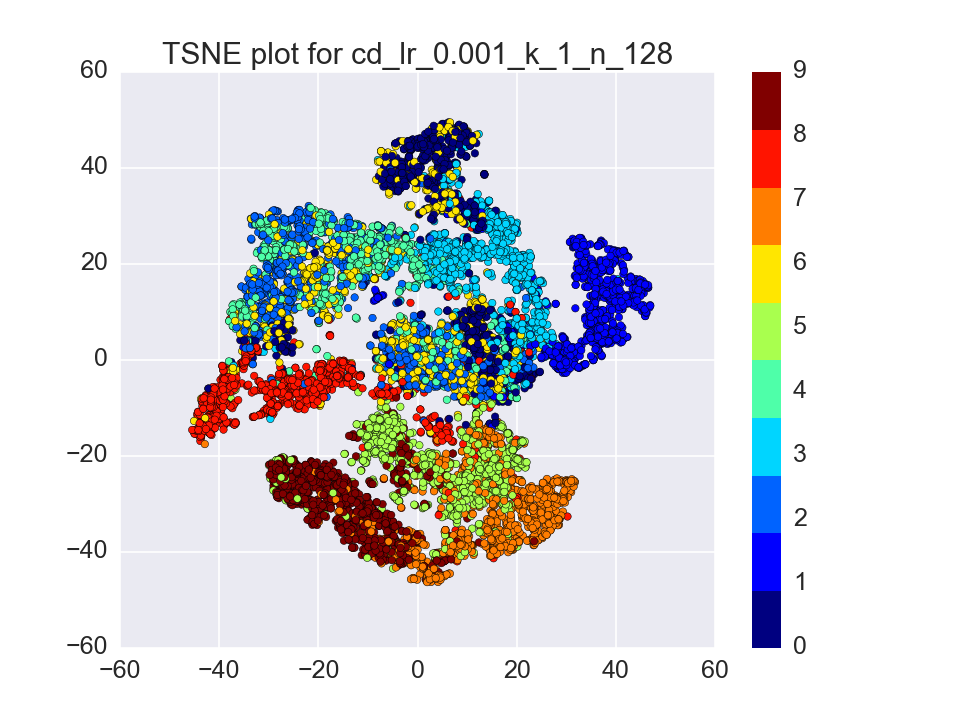
\includegraphics[scale=0.25]{cd_lr_0_001_k_1_n_128.png}
    \end{minipage} &
    \begin{minipage}{.3\textwidth}
      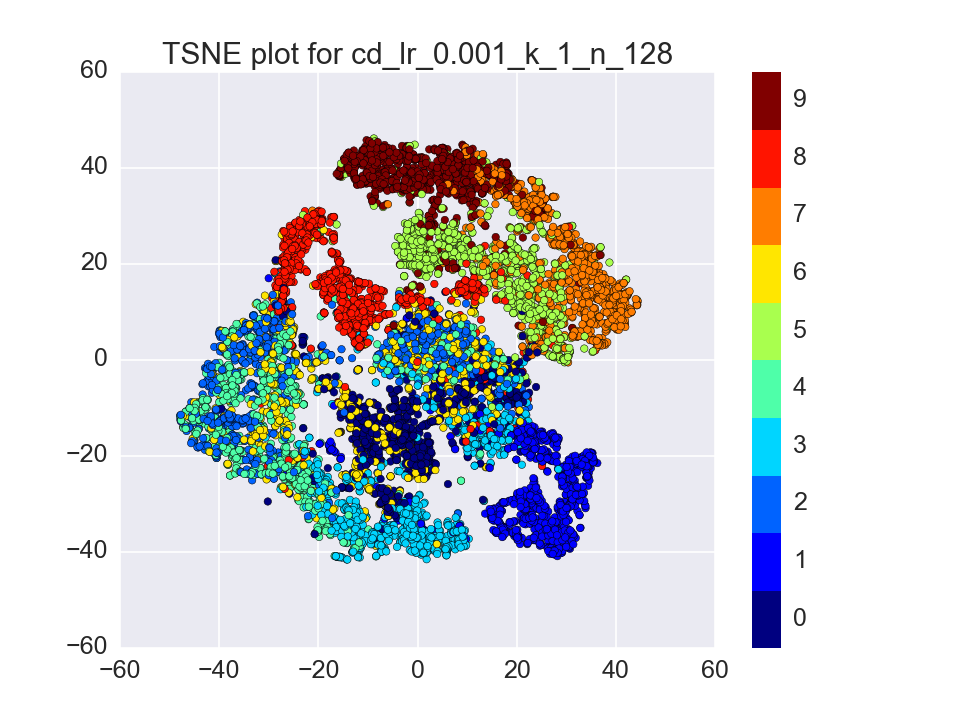
\includegraphics[scale=0.25]{test_cd_lr_0_001_k_1_n_128.png}
    \end{minipage}
    \\ \hline
    1e-3 & 128 & 2 &
    \begin{minipage}{.3\textwidth}
      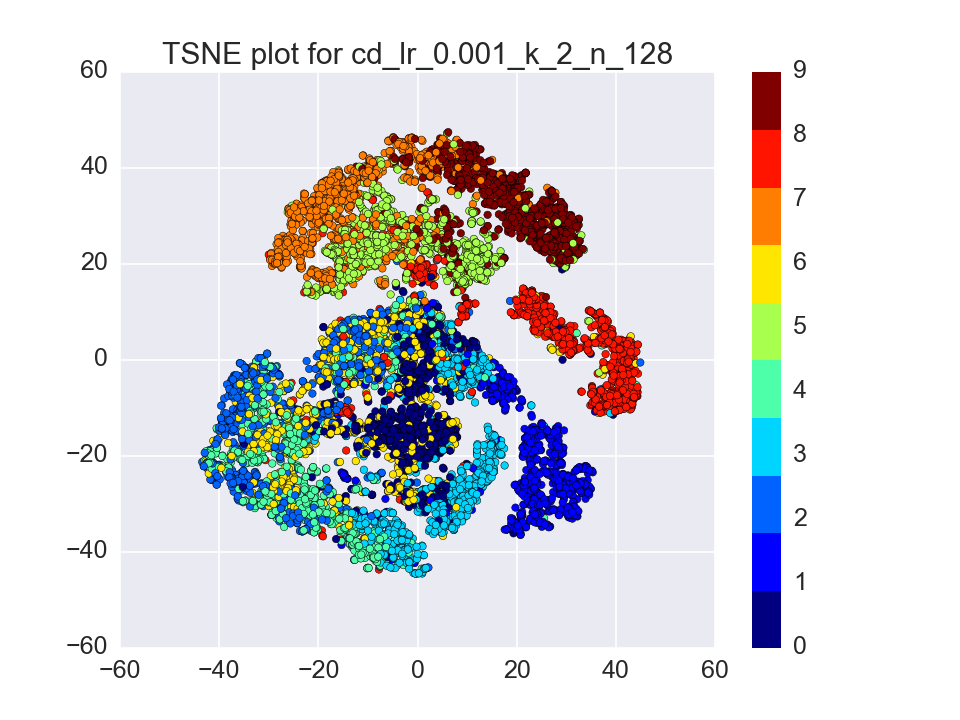
\includegraphics[scale=0.25]{cd_lr_0_001_k_2_n_128.png}
      %\includegraphics[width=\linewidth, height=60mm]{tiger}
    \end{minipage} &
    \begin{minipage}{.3\textwidth}
      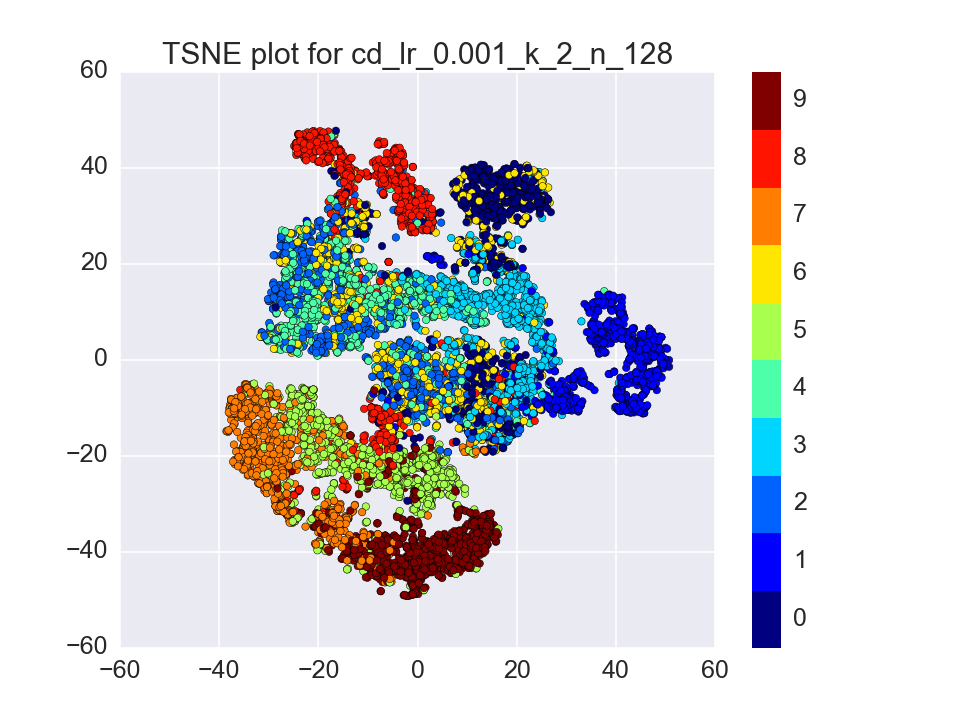
\includegraphics[scale=0.25]{test_cd_lr_0_001_k_2_n_128.png}
      %\includegraphics[width=\linewidth, height=60mm]{tiger}
    \end{minipage}
    \\ \hline
    1e-3 & 128 & 4 &
    \begin{minipage}{.3\textwidth}
      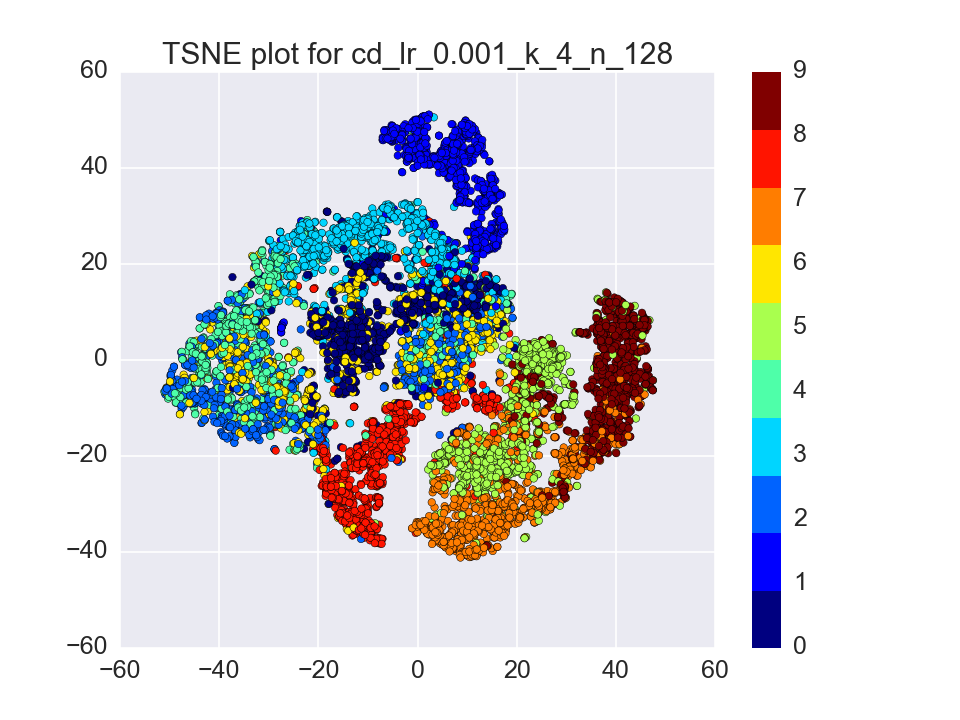
\includegraphics[scale=0.25]{cd_lr_0_001_k_4_n_128.png}
      %\includegraphics[width=\linewidth, height=60mm]{tiger}
    \end{minipage} &
    \begin{minipage}{.3\textwidth}
      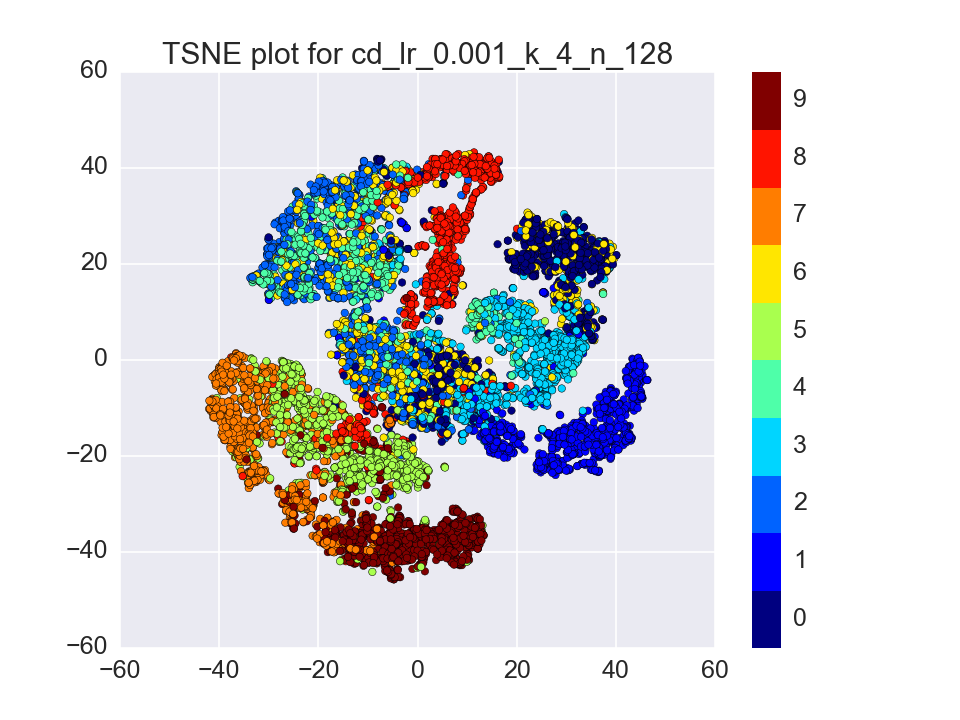
\includegraphics[scale=0.25]{test_cd_lr_0_001_k_4_n_128.png}
      %\includegraphics[width=\linewidth, height=60mm]{tiger}
    \end{minipage}
        \\ \hline
    1e-3 & 128 & 8 &
    \begin{minipage}{.3\textwidth}
      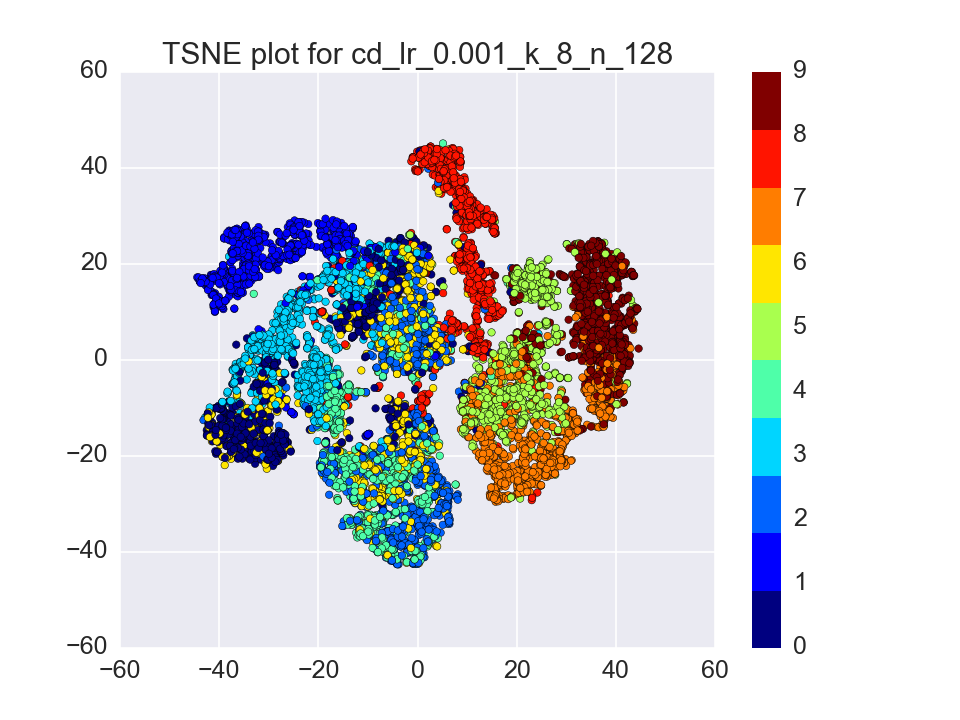
\includegraphics[scale=0.25]{cd_lr_0_001_k_8_n_128.png}
      %\includegraphics[width=\linewidth, height=60mm]{tiger}
    \end{minipage} &
    \begin{minipage}{.3\textwidth}
      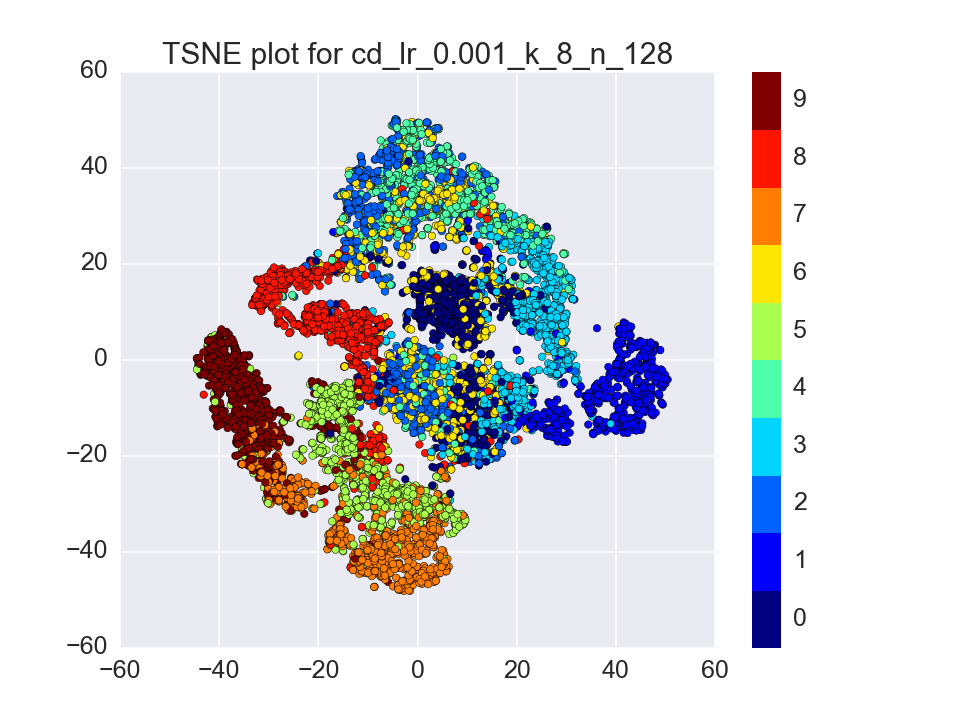
\includegraphics[scale=0.25]{test_cd_lr_0_001_k_8_n_128.png}
      %\includegraphics[width=\linewidth, height=60mm]{tiger}
    \end{minipage}
        \\ \hline
    1e-3 & 128 & 16 &
    \begin{minipage}{.3\textwidth}
      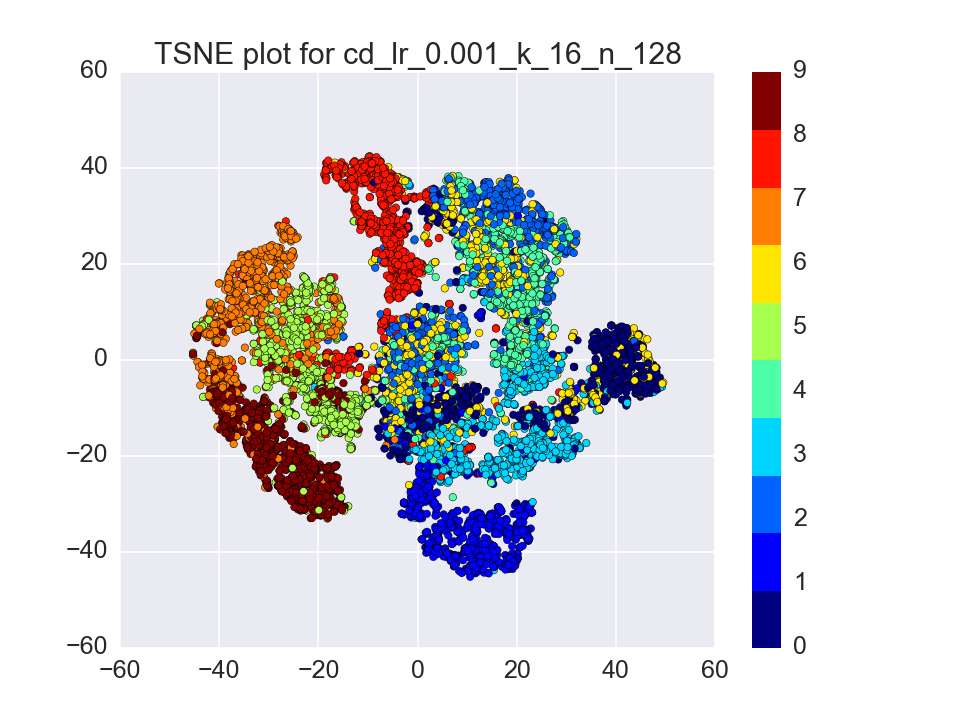
\includegraphics[scale=0.25]{cd_lr_0_001_k_16_n_128.png}
      %\includegraphics[width=\linewidth, height=60mm]{tiger}
    \end{minipage} &
    \begin{minipage}{.3\textwidth}
      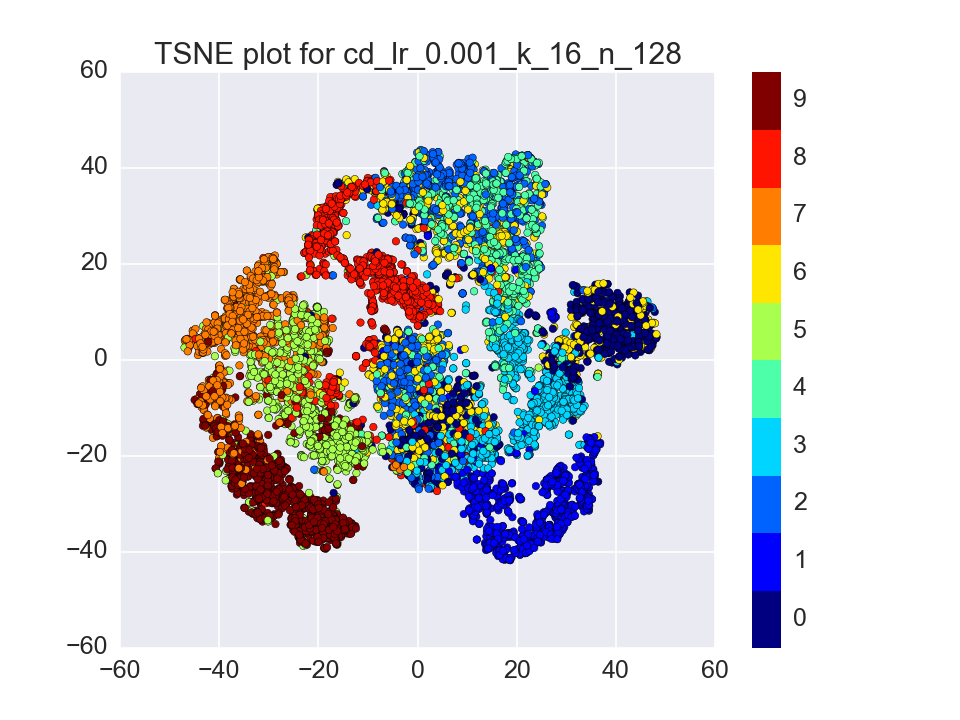
\includegraphics[scale=0.25]{test_cd_lr_0_001_k_16_n_128.png}
      %\includegraphics[width=\linewidth, height=60mm]{tiger}
    \end{minipage}
        \\ \hline
  \end{tabular}
\end{table}

\begin{table}[H]
  \centering
  \begin{tabular}{ | c | c | c | c || c |}
    \hline
    \textbf{lr} & \textbf{n} & \textbf{k} & \textbf{Train t-SNE} & \textbf{Test t-SNE}\\ \hline
    1e-3 & 128 & 32 &
    \begin{minipage}{.3\textwidth}
      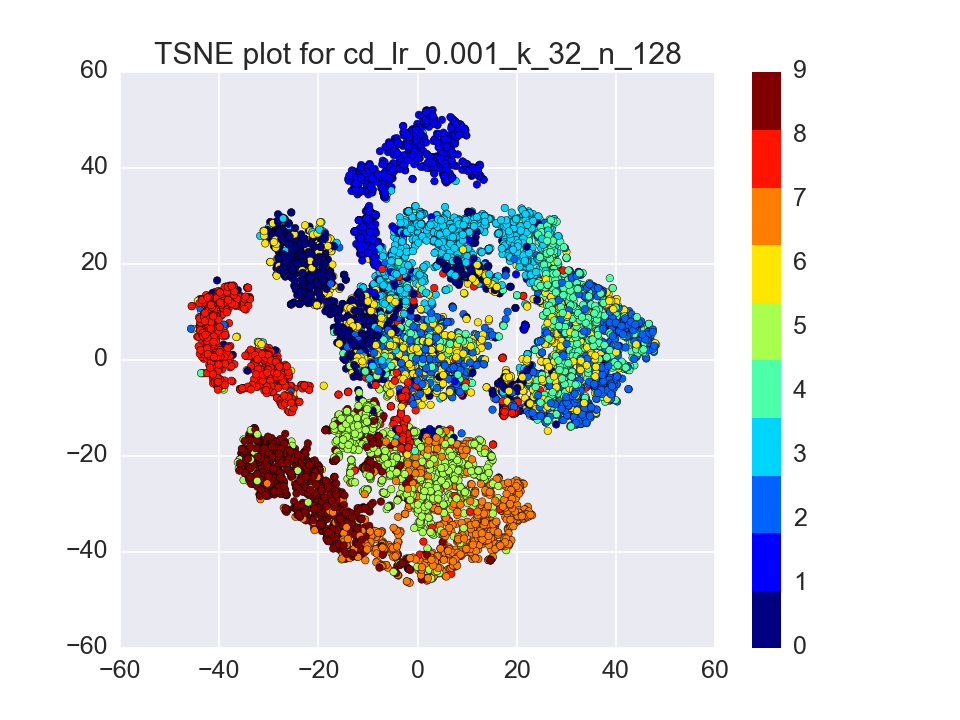
\includegraphics[scale=0.25]{cd_lr_0_001_k_32_n_128.png}
      %\includegraphics[width=\linewidth, height=60mm]{tiger}
    \end{minipage} &
    \begin{minipage}{.3\textwidth}
      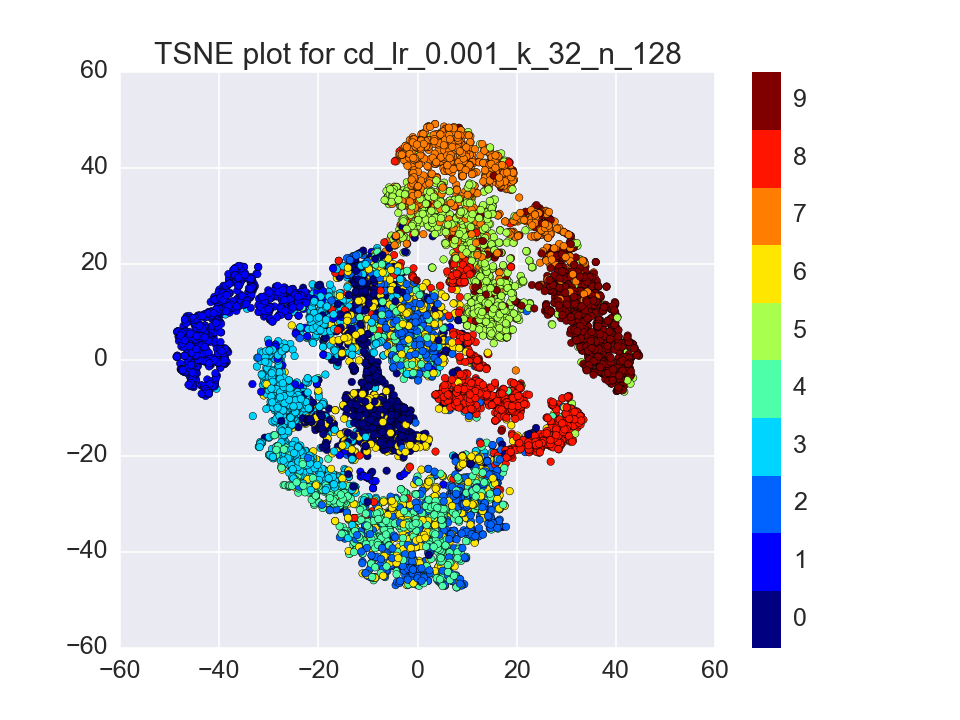
\includegraphics[scale=0.25]{test_cd_lr_0_001_k_32_n_128.png}
      %\includegraphics[width=\linewidth, height=60mm]{tiger}
    \end{minipage}
   \\ \hline
  \end{tabular}
\end{table}

\subsection{lr = 1e-3, n = 64}
\begin{table}[H]
  \centering
  \begin{tabular}{ | c | c | c | c || c |}
    \hline
    \textbf{lr} & \textbf{n} & \textbf{k} & \textbf{Train t-SNE} & \textbf{Test t-SNE} \\ \hline
    1e-3 & 64 & 1 &
    \begin{minipage}{.3\textwidth}
      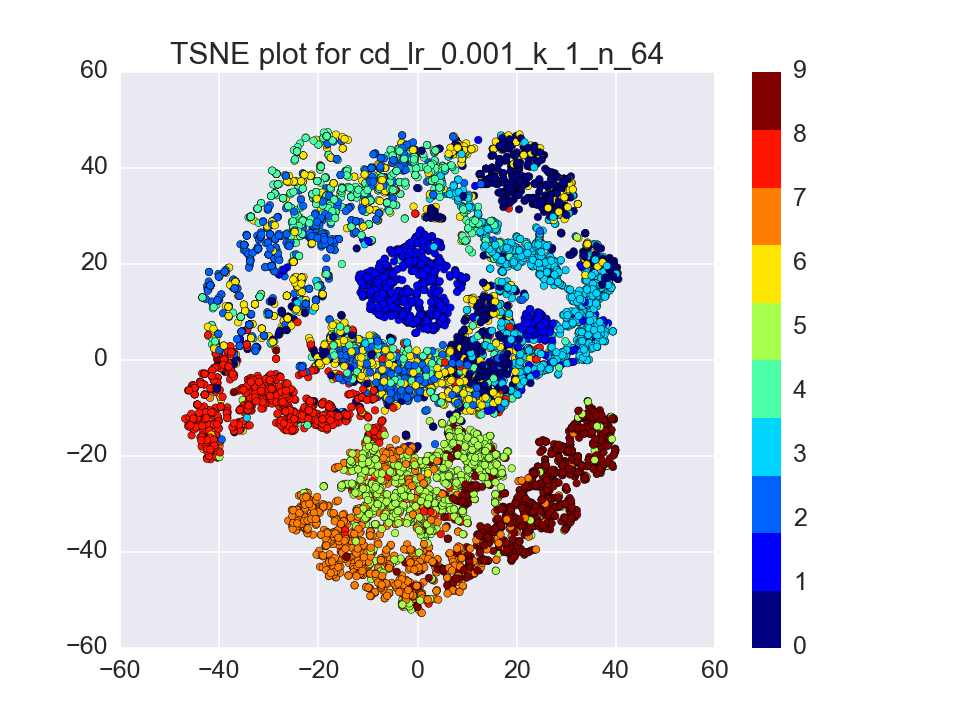
\includegraphics[scale=0.25]{cd_lr_0_001_k_1_n_64.png}
    \end{minipage} &
    \begin{minipage}{.3\textwidth}
      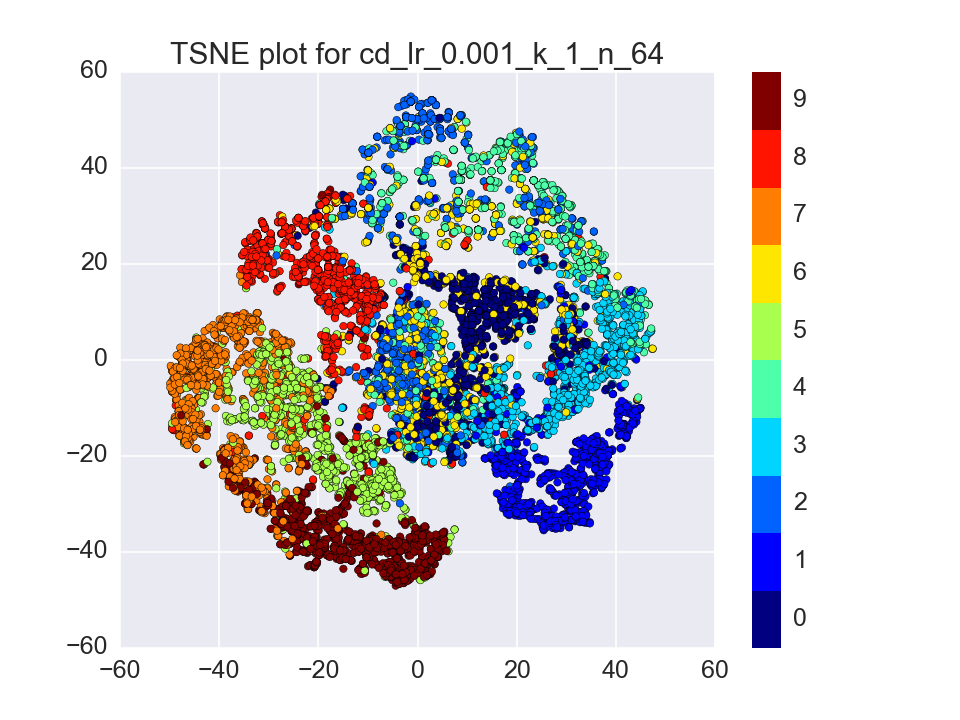
\includegraphics[scale=0.25]{test_cd_lr_0_001_k_1_n_64.png}
    \end{minipage}
    \\ \hline
    1e-3 & 64 & 2 &
    \begin{minipage}{.3\textwidth}
      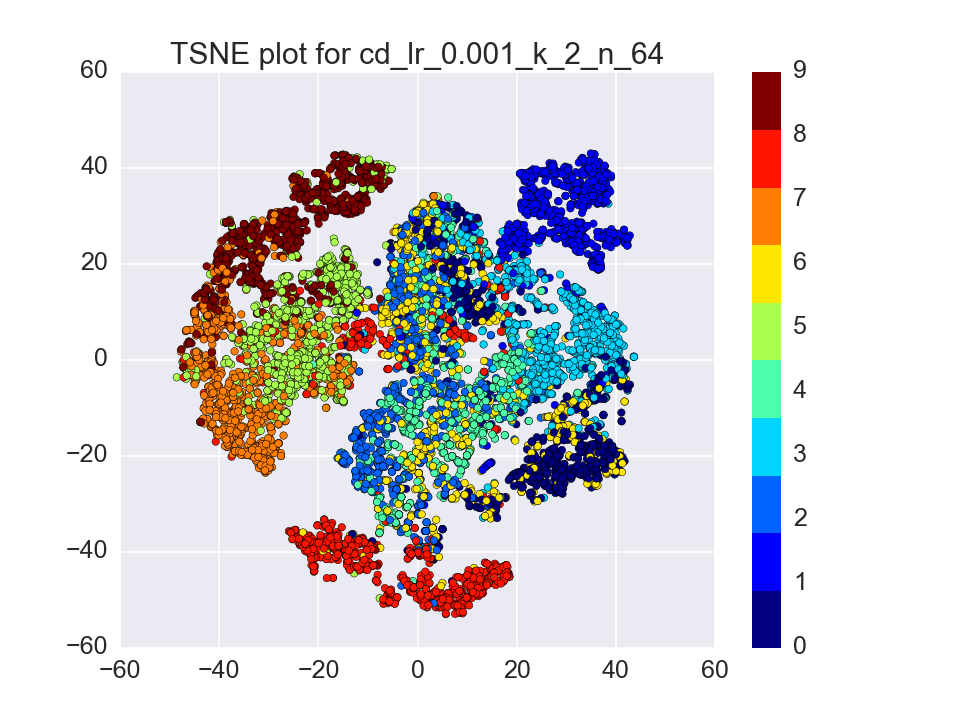
\includegraphics[scale=0.25]{cd_lr_0_001_k_2_n_64.png}
      %\includegraphics[width=\linewidth, height=60mm]{tiger}
    \end{minipage} &
    \begin{minipage}{.3\textwidth}
      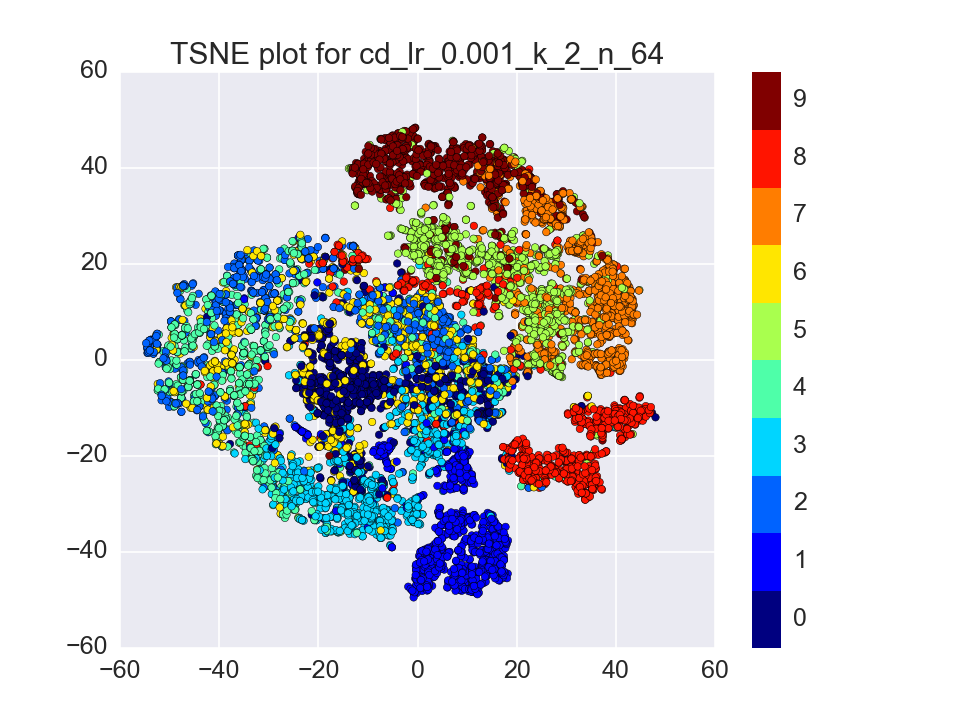
\includegraphics[scale=0.25]{test_cd_lr_0_001_k_2_n_64.png}
      %\includegraphics[width=\linewidth, height=60mm]{tiger}
    \end{minipage}
    \\ \hline
    1e-3 & 64 & 4 &
    \begin{minipage}{.3\textwidth}
      \includegraphics[scale=0.25]{cd_lr_0_001_k_4_n_64.png}
      %\includegraphics[width=\linewidth, height=60mm]{tiger}
    \end{minipage} &
    \begin{minipage}{.3\textwidth}
      \includegraphics[scale=0.25]{test_cd_lr_0_001_k_4_n_64.png}
      %\includegraphics[width=\linewidth, height=60mm]{tiger}
    \end{minipage}
        \\ \hline
  \end{tabular}
\end{table}

\begin{table}[H]
  \centering
  \begin{tabular}{ | c | c | c | c || c |}
    \hline
    \textbf{lr} & \textbf{n} & \textbf{k} & \textbf{Train t-SNE} & \textbf{Test t-SNE} \\ \hline 
    1e-3 & 64 & 8 &
    \begin{minipage}{.3\textwidth}
      \includegraphics[scale=0.25]{cd_lr_0_001_k_8_n_64.png}
      %\includegraphics[width=\linewidth, height=60mm]{tiger}
    \end{minipage} &
    \begin{minipage}{.3\textwidth}
      \includegraphics[scale=0.25]{test_cd_lr_0_001_k_8_n_64.png}
      %\includegraphics[width=\linewidth, height=60mm]{tiger}
    \end{minipage}
        \\ \hline
     1e-3 & 64 & 16 &
    \begin{minipage}{.3\textwidth}
      \includegraphics[scale=0.25]{cd_lr_0_001_k_16_n_64.png}
      %\includegraphics[width=\linewidth, height=60mm]{tiger}
    \end{minipage} &
    \begin{minipage}{.3\textwidth}
      \includegraphics[scale=0.25]{test_cd_lr_0_001_k_16_n_64.png}
      %\includegraphics[width=\linewidth, height=60mm]{tiger}
    \end{minipage}
        \\ \hline
    1e-3 & 64 & 32 &
    \begin{minipage}{.3\textwidth}
      \includegraphics[scale=0.25]{cd_lr_0_001_k_32_n_64.png}
      %\includegraphics[width=\linewidth, height=60mm]{tiger}
    \end{minipage} &
    \begin{minipage}{.3\textwidth}
      \includegraphics[scale=0.25]{test_cd_lr_0_001_k_32_n_64.png}
      %\includegraphics[width=\linewidth, height=60mm]{tiger}
    \end{minipage}
   \\ \hline
  \end{tabular}
\end{table}


\subsection{lr = 1e-4, n = 256}

\begin{table}[H]
  \centering
  \begin{tabular}{ | c | c | c | c || c |}
    \hline
    \textbf{lr} & \textbf{n} & \textbf{k} & \textbf{Train t-SNE} & \textbf{Test t-SNE}\\ \hline
    1e-4 & 256 & 1 &
    \begin{minipage}{.3\textwidth}
      \includegraphics[scale=0.25]{cd_lr_0_0001_k_1_n_256.png}
    \end{minipage} &
    \begin{minipage}{.3\textwidth}
      \includegraphics[scale=0.25]{test_cd_lr_0_0001_k_1_n_256.png}
    \end{minipage}
    \\ \hline
  \end{tabular}
\end{table}


\begin{table}[H]
  \centering
  \begin{tabular}{ | c | c | c | c || c |}
    \hline
    \textbf{lr} & \textbf{n} & \textbf{k} & \textbf{Train t-SNE} & \textbf{Test t-SNE}\\ \hline
    1e-4 & 256 & 2 &
    \begin{minipage}{.3\textwidth}
      \includegraphics[scale=0.25]{cd_lr_0_0001_k_2_n_256.png}
      %\includegraphics[width=\linewidth, height=60mm]{tiger}
    \end{minipage} &
    \begin{minipage}{.3\textwidth}
      \includegraphics[scale=0.25]{test_cd_lr_0_0001_k_2_n_256.png}
      %\includegraphics[width=\linewidth, height=60mm]{tiger}
    \end{minipage}
    \\ \hline
    1e-4 & 256 & 4 &
    \begin{minipage}{.3\textwidth}
      \includegraphics[scale=0.25]{cd_lr_0_0001_k_4_n_256.png}
      %\includegraphics[width=\linewidth, height=60mm]{tiger}
    \end{minipage} &
    \begin{minipage}{.3\textwidth}
      \includegraphics[scale=0.25]{test_cd_lr_0_0001_k_4_n_256.png}
      %\includegraphics[width=\linewidth, height=60mm]{tiger}
    \end{minipage}
        \\ \hline
    1e-4 & 256 & 8 &
    \begin{minipage}{.3\textwidth}
      \includegraphics[scale=0.25]{cd_lr_0_0001_k_8_n_256.png}
      %\includegraphics[width=\linewidth, height=60mm]{tiger}
    \end{minipage} &
    \begin{minipage}{.3\textwidth}
      \includegraphics[scale=0.25]{test_cd_lr_0_0001_k_8_n_256.png}
      %\includegraphics[width=\linewidth, height=60mm]{tiger}
    \end{minipage}
        \\ \hline
    1e-4 & 256 & 16 &
    \begin{minipage}{.3\textwidth}
      \includegraphics[scale=0.25]{cd_lr_0_0001_k_16_n_256.png}
      %\includegraphics[width=\linewidth, height=60mm]{tiger}
    \end{minipage} &
    \begin{minipage}{.3\textwidth}
      \includegraphics[scale=0.25]{test_cd_lr_0_0001_k_16_n_256.png}
      %\includegraphics[width=\linewidth, height=60mm]{tiger}
    \end{minipage}
        \\ \hline
    1e-4 & 256 & 32 &
    \begin{minipage}{.3\textwidth}
      \includegraphics[scale=0.25]{cd_lr_0_0001_k_32_n_256.png}
      %\includegraphics[width=\linewidth, height=60mm]{tiger}
    \end{minipage} &
    \begin{minipage}{.3\textwidth}
      \includegraphics[scale=0.25]{test_cd_lr_0_0001_k_32_n_256.png}
      %\includegraphics[width=\linewidth, height=60mm]{tiger}
    \end{minipage}
   \\ \hline
  \end{tabular}
\end{table}


\subsection{lr = 1e-4, n = 128}
\begin{table}[H]
  \centering
  \begin{tabular}{ | c | c | c | c || c |}
    \hline
    \textbf{lr} & \textbf{n} & \textbf{k} & \textbf{Train t-SNE} & \textbf{Test t-SNE}\\ \hline
    1e-4 & 128 & 1 &
    \begin{minipage}{.3\textwidth}
      \includegraphics[scale=0.25]{cd_lr_0_0001_k_1_n_128.png}
    \end{minipage} &
    \begin{minipage}{.3\textwidth}
      \includegraphics[scale=0.25]{test_cd_lr_0_0001_k_1_n_128.png}
    \end{minipage}
    \\ \hline
    1e-4 & 128 & 2 &
    \begin{minipage}{.3\textwidth}
      \includegraphics[scale=0.25]{cd_lr_0_0001_k_2_n_128.png}
      %\includegraphics[width=\linewidth, height=60mm]{tiger}
    \end{minipage} &
    \begin{minipage}{.3\textwidth}
      \includegraphics[scale=0.25]{test_cd_lr_0_0001_k_2_n_128.png}
      %\includegraphics[width=\linewidth, height=60mm]{tiger}
    \end{minipage}
    \\ \hline
    1e-4 & 128 & 4 &
    \begin{minipage}{.3\textwidth}
      \includegraphics[scale=0.25]{cd_lr_0_0001_k_4_n_128.png}
      %\includegraphics[width=\linewidth, height=60mm]{tiger}
    \end{minipage} &
    \begin{minipage}{.3\textwidth}
      \includegraphics[scale=0.25]{test_cd_lr_0_0001_k_4_n_128.png}
      %\includegraphics[width=\linewidth, height=60mm]{tiger}
    \end{minipage}
        \\ \hline
    1e-4 & 128 & 8 &
    \begin{minipage}{.3\textwidth}
      \includegraphics[scale=0.25]{cd_lr_0_0001_k_8_n_128.png}
      %\includegraphics[width=\linewidth, height=60mm]{tiger}
    \end{minipage} &
    \begin{minipage}{.3\textwidth}
      \includegraphics[scale=0.25]{test_cd_lr_0_0001_k_8_n_128.png}
      %\includegraphics[width=\linewidth, height=60mm]{tiger}
    \end{minipage}
        \\ \hline
    1e-4 & 128 & 16 &
    \begin{minipage}{.3\textwidth}
      \includegraphics[scale=0.25]{cd_lr_0_0001_k_16_n_128.png}
      %\includegraphics[width=\linewidth, height=60mm]{tiger}
    \end{minipage} &
    \begin{minipage}{.3\textwidth}
      \includegraphics[scale=0.25]{test_cd_lr_0_0001_k_16_n_128.png}
      %\includegraphics[width=\linewidth, height=60mm]{tiger}
    \end{minipage}
        \\ \hline
  \end{tabular}
\end{table}

\begin{table}[H]
  \centering
  \begin{tabular}{ | c | c | c | c || c |}
    \hline
    \textbf{lr} & \textbf{n} & \textbf{k} & \textbf{Train t-SNE} & \textbf{Test t-SNE}\\ \hline
    1e-4 & 128 & 32 &
    \begin{minipage}{.3\textwidth}
      \includegraphics[scale=0.25]{cd_lr_0_0001_k_32_n_128.png}
      %\includegraphics[width=\linewidth, height=60mm]{tiger}
    \end{minipage} &
    \begin{minipage}{.3\textwidth}
      \includegraphics[scale=0.25]{test_cd_lr_0_0001_k_32_n_128.png}
      %\includegraphics[width=\linewidth, height=60mm]{tiger}
    \end{minipage}
   \\ \hline
  \end{tabular}
\end{table}

\subsection{lr = 1e-4, n = 64}

\begin{table}[H]
  \centering
  \begin{tabular}{ | c | c | c | c || c |}
    \hline
    \textbf{lr} & \textbf{n} & \textbf{k} & \textbf{Train t-SNE} & \textbf{Test t-SNE} \\ \hline
    1e-4 & 64 & 1 &
    \begin{minipage}{.3\textwidth}
      \includegraphics[scale=0.25]{cd_lr_0_0001_k_1_n_64.png}
    \end{minipage} &
    \begin{minipage}{.3\textwidth}
      \includegraphics[scale=0.25]{test_cd_lr_0_0001_k_1_n_64.png}
    \end{minipage}
    \\ \hline
    1e-4 & 64 & 2 &
    \begin{minipage}{.3\textwidth}
      \includegraphics[scale=0.25]{cd_lr_0_0001_k_2_n_64.png}
      %\includegraphics[width=\linewidth, height=60mm]{tiger}
    \end{minipage} &
    \begin{minipage}{.3\textwidth}
      \includegraphics[scale=0.25]{test_cd_lr_0_0001_k_2_n_64.png}
      %\includegraphics[width=\linewidth, height=60mm]{tiger}
    \end{minipage}
    \\ \hline
    1e-4 & 64 & 4 &
    \begin{minipage}{.3\textwidth}
      \includegraphics[scale=0.25]{cd_lr_0_0001_k_4_n_64.png}
      %\includegraphics[width=\linewidth, height=60mm]{tiger}
    \end{minipage} &
    \begin{minipage}{.3\textwidth}
      \includegraphics[scale=0.25]{test_cd_lr_0_0001_k_4_n_64.png}
      %\includegraphics[width=\linewidth, height=60mm]{tiger}
    \end{minipage}
        \\ \hline
  \end{tabular}
\end{table}

\begin{table}[H]
  \centering
  \begin{tabular}{ | c | c | c | c || c |}
    \hline
    \textbf{lr} & \textbf{n} & \textbf{k} & \textbf{Train t-SNE} & \textbf{Test t-SNE} \\ \hline
    1e-4 & 64 & 8 &
    \begin{minipage}{.3\textwidth}
      \includegraphics[scale=0.25]{cd_lr_0_0001_k_8_n_64.png}
      %\includegraphics[width=\linewidth, height=60mm]{tiger}
    \end{minipage} &
    \begin{minipage}{.3\textwidth}
      \includegraphics[scale=0.25]{test_cd_lr_0_0001_k_8_n_64.png}
      %\includegraphics[width=\linewidth, height=60mm]{tiger}
    \end{minipage}
        \\ \hline
    1e-4 & 64 & 16 &
    \begin{minipage}{.3\textwidth}
      \includegraphics[scale=0.25]{cd_lr_0_0001_k_16_n_64.png}
      %\includegraphics[width=\linewidth, height=60mm]{tiger}
    \end{minipage} &
    \begin{minipage}{.3\textwidth}
      \includegraphics[scale=0.25]{test_cd_lr_0_0001_k_16_n_64.png}
      %\includegraphics[width=\linewidth, height=60mm]{tiger}
    \end{minipage}
        \\ \hline
    1e-4 & 64 & 32 &
    \begin{minipage}{.3\textwidth}
      \includegraphics[scale=0.25]{cd_lr_0_0001_k_32_n_64.png}
      %\includegraphics[width=\linewidth, height=60mm]{tiger}
    \end{minipage} &
    \begin{minipage}{.3\textwidth}
      \includegraphics[scale=0.25]{test_cd_lr_0_0001_k_32_n_64.png}
      %\includegraphics[width=\linewidth, height=60mm]{tiger}
    \end{minipage}
   \\ \hline
  \end{tabular}
\end{table}

On observing the TSNE plots we note that the points mostly cluster according to their class. Similar classes tend to overlap. The tabulations are all for 20 epochs, after which, the based models were restored and trained using early stopping. On increasing the n value, we note an decrease in reconstruction error. (steeper for smaller values of n, and magnitude of decrease decreases as we increase the n value. Naturally, this makes sense, as in the limiting case of n=784, we achieve perfect reconstruction. At lower n values, we are restricting the hidden variables ability to capture information about the images. 
Around n=64 we observe reconstruction errors in the range of 80s, at n=128 around 60s, and further decreases to around 50s for n=256.

\subsection{lr = (1e-5, 1e-6), n = 128}

\begin{table}[H]
  \centering
  \begin{tabular}{ | c | c | c | c || c |}
    \hline
    \textbf{lr} & \textbf{n} & \textbf{k} & \textbf{Train t-SNE} & \textbf{Test t-SNE} \\ \hline
    1e-5 & 128 & 1 &
    \begin{minipage}{.3\textwidth}
      \includegraphics[scale=0.25]{cd_lr_1e-05_k_1_n_128.png}
    \end{minipage} &
    \begin{minipage}{.3\textwidth}
      \includegraphics[scale=0.25]{test_cd_lr_1e-05_k_1_n_128.png}
    \end{minipage}
    \\ \hline
    1e-5 & 128 & 2 &
    \begin{minipage}{.3\textwidth}
      \includegraphics[scale=0.25]{cd_lr_1e-05_k_2_n_128.png}
      %\includegraphics[width=\linewidth, height=60mm]{tiger}
    \end{minipage} &
    \begin{minipage}{.3\textwidth}
      \includegraphics[scale=0.25]{test_cd_lr_1e-05_k_2_n_128.png}
      %\includegraphics[width=\linewidth, height=60mm]{tiger}
    \end{minipage}
    \\ \hline
    1e-6 & 128 & 1 &
    \begin{minipage}{.3\textwidth}
      \includegraphics[scale=0.25]{cd_lr_1e-06_k_1_n_128.png}
      %\includegraphics[width=\linewidth, height=60mm]{tiger}
    \end{minipage} &
    \begin{minipage}{.3\textwidth}
      \includegraphics[scale=0.25]{test_cd_lr_1e-06_k_1_n_128.png}
      %\includegraphics[width=\linewidth, height=60mm]{tiger}
    \end{minipage}
        \\ \hline
     1e-6 & 128 & 2 &
    \begin{minipage}{.3\textwidth}
      \includegraphics[scale=0.25]{cd_lr_1e-06_k_2_n_128.png}
      %\includegraphics[width=\linewidth, height=60mm]{tiger}
    \end{minipage} &
    \begin{minipage}{.3\textwidth}
      \includegraphics[scale=0.25]{test_cd_lr_1e-06_k_2_n_128.png}
      %\includegraphics[width=\linewidth, height=60mm]{tiger}
    \end{minipage}
        \\ \hline
  \end{tabular}
\end{table}

As the t-SNE plots were not very well separated for the cases were learning rate was less that 1e-4, such cases were avoided further on while plotting.

%-------------------------------------------------------------------------------
% Question 2
%-------------------------------------------------------------------------------
\section{Effects of k on Gibbs Chain}
\begin{table}[H]
  \centering
  \begin{tabular}{ | c | c | c | c |}
    \hline
    \textbf{lr} & \textbf{n} & \textbf{Train Plot} & \textbf{Test Plot} \\ \hline
    1e-3 & 256 &
    \begin{minipage}{.3\textwidth}
    \includegraphics[scale=0.25]{train_cd_lr_0_001_n_256.png}
    \end{minipage} &
    \begin{minipage}{.3\textwidth}
      \includegraphics[scale=0.25]{cd_lr_0_001_n_256.png}
    \end{minipage}
    \\ \hline
    1e-3 & 128 &
    \begin{minipage}{.3\textwidth}
    \includegraphics[scale=0.2]{train_cd_lr_0_001_n_128.png}
    \end{minipage} &
    \begin{minipage}{.3\textwidth}
      \includegraphics[scale=0.2]{cd_lr_0_001_n_128.png}
    \end{minipage}
    \\ \hline
    1e-3 & 64 &
    \begin{minipage}{.3\textwidth}
      \includegraphics[scale=0.25]{train_cd_lr_0_001_n_64.png}
    \end{minipage} &
    \begin{minipage}{.3\textwidth}
      \includegraphics[scale=0.25]{cd_lr_0_001_n_64.png}
    \end{minipage}
    \\ \hline
  \end{tabular}
\end{table}


\begin{table}[H]
  \centering
  \begin{tabular}{ | c | c | c | c |}
    \hline
    \textbf{lr} & \textbf{n} & \textbf{Train Plot} & \textbf{Test Plot} \\ \hline
    1e-4 & 256 &
    \begin{minipage}{.3\textwidth}
      \includegraphics[scale=0.25]{train_cd_lr_0_0001_n_256.png}
    \end{minipage} &
    \begin{minipage}{.3\textwidth}
      \includegraphics[scale=0.25]{cd_lr_0_0001_n_256.png}
    \end{minipage}
    \\ \hline
    1e-4 & 128 &
    \begin{minipage}{.3\textwidth}
      \includegraphics[scale=0.2]{train_cd_lr_0_0001_n_128.png}
    \end{minipage} &
    \begin{minipage}{.3\textwidth}
      \includegraphics[scale=0.2]{cd_lr_0_0001_n_128.png}
    \end{minipage}
    \\ \hline
    1e-4 & 64 &
    \begin{minipage}{.3\textwidth}
      \includegraphics[scale=0.25]{train_cd_lr_0_0001_n_64.png}
    \end{minipage} &
    \begin{minipage}{.3\textwidth}
      \includegraphics[scale=0.25]{cd_lr_0_0001_n_64.png}
    \end{minipage}
    \\ \hline
  \end{tabular}
\end{table}


\begin{table}[H]
  \centering
  \begin{tabular}{ | c | c | c | c |}
    \hline
    \textbf{lr} & \textbf{n} & \textbf{Train Plot} & \textbf{Test Plot} \\ \hline
    1e-5 & 256 &
    \begin{minipage}{.3\textwidth}
      \includegraphics[scale=0.25]{train_cd_lr_0_00001_n_256.png}
    \end{minipage} &
    \begin{minipage}{.3\textwidth}
      \includegraphics[scale=0.25]{cd_lr_0_00001_n_256.png}
    \end{minipage}
    \\ \hline
    1e-5 & 128 &
    \begin{minipage}{.3\textwidth}
      \includegraphics[scale=0.2]{train_cd_lr_0_00001_n_128.png}
    \end{minipage} &
    \begin{minipage}{.3\textwidth}
      \includegraphics[scale=0.2]{cd_lr_0_00001_n_128.png}
    \end{minipage}
    \\ \hline
    1e-5 & 64 &
    \begin{minipage}{.3\textwidth}
      \includegraphics[scale=0.25]{train_cd_lr_0_00001_n_64.png}
    \end{minipage} &
    \begin{minipage}{.3\textwidth}
      \includegraphics[scale=0.25]{cd_lr_0_00001_n_64.png}
    \end{minipage}
    \\ \hline
  \end{tabular}
\end{table}

We note a non-linear trend on using different k values (note this could be because we trained it to a certain fixed point for all models) . Ideally as number of iterations tends to infinity, we should expect them all to arrive at similar models. The rate of convergence depends on k. We notice faster convergence for moderate k values (in terms of time and iterations) . If we fix the number of iterations , larger k values perform better, however, there is a tradeoff, as the amount of time taken for each step increases with larger k.
%-------------------------------------------------------------------------------
% Question 3
%-------------------------------------------------------------------------------
\section{Plots of samples generated by Gibbs Chain}
The best model that was obtained using a learning rate of 0.001 and hidden representation of size 256 and k value as 2 (as can be seen from the plot above), was ran for 40 epochs and the reconstructed images of certain validation samples were saved as examined as follows :

\begin{table}[H]
  \centering
  \begin{tabular}{  c  c  c  c  c  c }
    \textbf{Original} & \textbf{1 epoch} & \textbf{2 epoch} & \textbf{4 epoch} & \textbf{16 epoch}  & \textbf{40 epoch} \\ 
    \begin{minipage}{.15\textwidth}
      \includegraphics[scale=0.2]{BM_avisual.png}
    \end{minipage} & 
    \begin{minipage}{.15\textwidth}
      \includegraphics[scale=0.2]{BM_a1.png}
    \end{minipage} &
    \begin{minipage}{.15\textwidth}
      \includegraphics[scale=0.2]{BM_a2.png}
    \end{minipage} &
    \begin{minipage}{.15\textwidth}
      \includegraphics[scale=0.2]{BM_a4.png}
    \end{minipage} &
    \begin{minipage}{.15\textwidth}
      \includegraphics[scale=0.2]{BM_a16.png}
    \end{minipage} &
    \begin{minipage}{.15\textwidth}
      \includegraphics[scale=0.2]{BM_a40.png}
    \end{minipage} \\ 
    \begin{minipage}{.15\textwidth}
      \includegraphics[scale=0.2]{BM_bvisual.png}
    \end{minipage} & 
    \begin{minipage}{.15\textwidth}
      \includegraphics[scale=0.2]{BM_b1.png}
    \end{minipage} &
    \begin{minipage}{.15\textwidth}
      \includegraphics[scale=0.2]{BM_b2.png}
    \end{minipage} &
    \begin{minipage}{.15\textwidth}
      \includegraphics[scale=0.2]{BM_b4.png}
    \end{minipage} &
    \begin{minipage}{.15\textwidth}
      \includegraphics[scale=0.2]{BM_b16.png}
    \end{minipage} &
    \begin{minipage}{.15\textwidth}
      \includegraphics[scale=0.2]{BM_b40.png}
    \end{minipage} \\ 
    \begin{minipage}{.15\textwidth}
      \includegraphics[scale=0.2]{BM_cvisual.png}
    \end{minipage} & 
    \begin{minipage}{.15\textwidth}
      \includegraphics[scale=0.2]{BM_c1.png}
    \end{minipage} &
    \begin{minipage}{.15\textwidth}
      \includegraphics[scale=0.2]{BM_c2.png}
    \end{minipage} &
    \begin{minipage}{.15\textwidth}
      \includegraphics[scale=0.2]{BM_c4.png}
    \end{minipage} &
    \begin{minipage}{.15\textwidth}
      \includegraphics[scale=0.2]{BM_c16.png}
    \end{minipage} &
    \begin{minipage}{.15\textwidth}
      \includegraphics[scale=0.2]{BM_c40.png}
    \end{minipage} \\ 
    \begin{minipage}{.15\textwidth}
      \includegraphics[scale=0.2]{BM_dvisual.png}
    \end{minipage} & 
    \begin{minipage}{.15\textwidth}
      \includegraphics[scale=0.2]{BM_d1.png}
    \end{minipage} &
    \begin{minipage}{.15\textwidth}
      \includegraphics[scale=0.2]{BM_d2.png}
    \end{minipage} &
    \begin{minipage}{.15\textwidth}
      \includegraphics[scale=0.2]{BM_d4.png}
    \end{minipage} &
    \begin{minipage}{.15\textwidth}
      \includegraphics[scale=0.2]{BM_d16.png}
    \end{minipage} &
    \begin{minipage}{.15\textwidth}
      \includegraphics[scale=0.2]{BM_d40.png}
    \end{minipage} \\ 
    \begin{minipage}{.15\textwidth}
      \includegraphics[scale=0.2]{BM_evisual.png}
    \end{minipage} & 
    \begin{minipage}{.15\textwidth}
      \includegraphics[scale=0.2]{BM_e1.png}
    \end{minipage} &
    \begin{minipage}{.15\textwidth}
      \includegraphics[scale=0.2]{BM_e2.png}
    \end{minipage} &
    \begin{minipage}{.15\textwidth}
      \includegraphics[scale=0.2]{BM_e4.png}
    \end{minipage} &
    \begin{minipage}{.15\textwidth}
      \includegraphics[scale=0.2]{BM_e16.png}
    \end{minipage} &
    \begin{minipage}{.15\textwidth}
      \includegraphics[scale=0.2]{BM_e40.png}
    \end{minipage} \\ 
    \begin{minipage}{.15\textwidth}
      \includegraphics[scale=0.2]{BM_fvisual.png}
    \end{minipage} & 
    \begin{minipage}{.15\textwidth}
      \includegraphics[scale=0.2]{BM_f1.png}
    \end{minipage} &
    \begin{minipage}{.15\textwidth}
      \includegraphics[scale=0.2]{BM_f2.png}
    \end{minipage} &
    \begin{minipage}{.15\textwidth}
      \includegraphics[scale=0.2]{BM_f4.png}
    \end{minipage} &
    \begin{minipage}{.15\textwidth}
      \includegraphics[scale=0.2]{BM_f16.png}
    \end{minipage} &
    \begin{minipage}{.15\textwidth}
      \includegraphics[scale=0.2]{BM_f40.png}
    \end{minipage}
  \end{tabular}
\end{table}

The corresponding hidden representations of the images is as shown below :

\begin{table}[H]
  \centering
  \begin{tabular}{  c  c  c  c  c  c }
    \begin{minipage}{.15\textwidth}
      \includegraphics[scale=0.2]{BM_ahidden.png}
    \end{minipage} &
    \begin{minipage}{.15\textwidth}
      \includegraphics[scale=0.2]{BM_bhidden.png}
    \end{minipage} &
    \begin{minipage}{.15\textwidth}
      \includegraphics[scale=0.2]{BM_chidden.png}
    \end{minipage} &
    \begin{minipage}{.15\textwidth}
      \includegraphics[scale=0.2]{BM_dhidden.png}
    \end{minipage}&
    \begin{minipage}{.15\textwidth}
      \includegraphics[scale=0.2]{BM_ehidden.png}
    \end{minipage} &
    \begin{minipage}{.15\textwidth}
      \includegraphics[scale=0.2]{BM_fhidden.png}
    \end{minipage}
  \end{tabular}
\end{table}


The average reconstruction error for train and validation datasets were recorded after every 5000 steps to measure convergence.
\begin{center}
\includegraphics[scale=0.5]{cost_train_lr_0_001_k_1_n_256.png}
\end{center}
\begin{center}
\includegraphics[scale=0.5]{cost_val_lr_0_001_k_1_n_256.png}
\end{center}

Initially the sampled images are meaningless, but over time/iterations, they start resembling blurry versions of the images from the training data, and around convergence they look like very convincing samples from the provided data.\\\\
As can be seen from the above graph, the reduction in reconstruction error is quite small beyond $100 \times 5000$ iterations. Hence, the m value was fixed to be that and the reconstructed images used while training was plotted on an $8 \times 8$ grid.

\begin{figure}[H]
\begin{tabular}{cccccccc}
  \includegraphics[width=0.1\linewidth]{qn2_i_0.png} &   \includegraphics[width=0.1\linewidth]{qn2_i_1.png} &
  \includegraphics[width=0.1\linewidth]{qn2_i_2.png} &   \includegraphics[width=0.1\linewidth]{qn2_i_3.png} &
  \includegraphics[width=0.1\linewidth]{qn2_i_4.png} &   \includegraphics[width=0.1\linewidth]{qn2_i_5.png} &
  \includegraphics[width=0.1\linewidth]{qn2_i_6.png} &   \includegraphics[width=0.1\linewidth]{qn2_i_7.png} \\
  \includegraphics[width=0.1\linewidth]{qn2_i_8.png} &   \includegraphics[width=0.1\linewidth]{qn2_i_9.png} &
  \includegraphics[width=0.1\linewidth]{qn2_i_10.png} &   \includegraphics[width=0.1\linewidth]{qn2_i_11.png} &
  \includegraphics[width=0.1\linewidth]{qn2_i_12.png} &   \includegraphics[width=0.1\linewidth]{qn2_i_13.png} &
  \includegraphics[width=0.1\linewidth]{qn2_i_14.png} &   \includegraphics[width=0.1\linewidth]{qn2_i_15.png} \\
  \includegraphics[width=0.1\linewidth]{qn2_i_16.png} &   \includegraphics[width=0.1\linewidth]{qn2_i_17.png} &
  \includegraphics[width=0.1\linewidth]{qn2_i_18.png} &   \includegraphics[width=0.1\linewidth]{qn2_i_19.png} &
  \includegraphics[width=0.1\linewidth]{qn2_i_20.png} &   \includegraphics[width=0.1\linewidth]{qn2_i_21.png} &
  \includegraphics[width=0.1\linewidth]{qn2_i_22.png} &   \includegraphics[width=0.1\linewidth]{qn2_i_23.png} \\
  \includegraphics[width=0.1\linewidth]{qn2_i_24.png} &   \includegraphics[width=0.1\linewidth]{qn2_i_25.png} &
  \includegraphics[width=0.1\linewidth]{qn2_i_26.png} &   \includegraphics[width=0.1\linewidth]{qn2_i_27.png} &
  \includegraphics[width=0.1\linewidth]{qn2_i_28.png} &   \includegraphics[width=0.1\linewidth]{qn2_i_29.png} &
  \includegraphics[width=0.1\linewidth]{qn2_i_30.png} &   \includegraphics[width=0.1\linewidth]{qn2_i_31.png} \\
  \includegraphics[width=0.1\linewidth]{qn2_i_32.png} &   \includegraphics[width=0.1\linewidth]{qn2_i_33.png} &
  \includegraphics[width=0.1\linewidth]{qn2_i_34.png} &   \includegraphics[width=0.1\linewidth]{qn2_i_35.png} &
  \includegraphics[width=0.1\linewidth]{qn2_i_36.png} &   \includegraphics[width=0.1\linewidth]{qn2_i_37.png} &
  \includegraphics[width=0.1\linewidth]{qn2_i_38.png} &   \includegraphics[width=0.1\linewidth]{qn2_i_39.png} \\
  \includegraphics[width=0.1\linewidth]{qn2_i_40.png} &   \includegraphics[width=0.1\linewidth]{qn2_i_41.png} &
  \includegraphics[width=0.1\linewidth]{qn2_i_42.png} &   \includegraphics[width=0.1\linewidth]{qn2_i_43.png} &
  \includegraphics[width=0.1\linewidth]{qn2_i_44.png} &   \includegraphics[width=0.1\linewidth]{qn2_i_45.png} &
  \includegraphics[width=0.1\linewidth]{qn2_i_46.png} &   \includegraphics[width=0.1\linewidth]{qn2_i_47.png} \\
  \includegraphics[width=0.1\linewidth]{qn2_i_48.png} &   \includegraphics[width=0.1\linewidth]{qn2_i_49.png} &
  \includegraphics[width=0.1\linewidth]{qn2_i_50.png} &   \includegraphics[width=0.1\linewidth]{qn2_i_51.png} &
  \includegraphics[width=0.1\linewidth]{qn2_i_52.png} &   \includegraphics[width=0.1\linewidth]{qn2_i_53.png} &
  \includegraphics[width=0.1\linewidth]{qn2_i_54.png} &   \includegraphics[width=0.1\linewidth]{qn2_i_55.png} \\
  \includegraphics[width=0.1\linewidth]{qn2_i_56.png} &   \includegraphics[width=0.1\linewidth]{qn2_i_57.png} &
  \includegraphics[width=0.1\linewidth]{qn2_i_58.png} &   \includegraphics[width=0.1\linewidth]{qn2_i_59.png} &
  \includegraphics[width=0.1\linewidth]{qn2_i_60.png} &   \includegraphics[width=0.1\linewidth]{qn2_i_61.png} &
  \includegraphics[width=0.1\linewidth]{qn2_i_62.png} &   \includegraphics[width=0.1\linewidth]{qn2_i_63.png} \\
\end{tabular}
\end{figure}

%-------------------------------------------------------------------------------
% Question 4
%-------------------------------------------------------------------------------
\section{Gibbs Sampling}
Withing the first 100 iterations ,(when sampled to large k values around 1000) we started getting meaningful images. As we approach convergence, the number of time steps required to get meaningful images decreases .(this is because our weights and biases are accurate, and we are quickly able to converge to the true distribution even after starting form a random point.\\\\
Despite starting from a random v value, we were able to achieve the following reconstructions for it during the training process :
\begin{figure}[H]
\begin{tabular}{cccccccc}
  \includegraphics[width=0.15\linewidth]{q3_1.png} &   \includegraphics[width=0.15\linewidth]{q3_2.png} &
  \includegraphics[width=0.15\linewidth]{q3_3.png} &   \includegraphics[width=0.15\linewidth]{q3_4.png} &
  \includegraphics[width=0.15\linewidth]{q3_5.png} &   \includegraphics[width=0.15\linewidth]{q3_6.png} \\
\end{tabular}
\end{figure}
Hence, we decided to go with the same random v and analyse the reconstruction with varying values of k and number of iterations.

\begin{figure}[H]
\begin{tabular}{cccccccc}
	\multicolumn{6}{c}{k decreases $\longleftarrow$} \\
	\multicolumn{6}{c}{iterations increases $\longrightarrow$} \\
  \includegraphics[width=0.15\linewidth]{1.png} &   \includegraphics[width=0.15\linewidth]{2.png} &
  \includegraphics[width=0.15\linewidth]{3.png} &   \includegraphics[width=0.15\linewidth]{4.png} &
  \includegraphics[width=0.15\linewidth]{5.png} &   \includegraphics[width=0.15\linewidth]{6.png}  \\
  \includegraphics[width=0.15\linewidth]{7.png} &   \includegraphics[width=0.15\linewidth]{8.png} &
  \includegraphics[width=0.15\linewidth]{9.png} &   \includegraphics[width=0.15\linewidth]{10.png} &
  \includegraphics[width=0.15\linewidth]{11.png} &   \includegraphics[width=0.15\linewidth]{12.png} \\
  \includegraphics[width=0.15\linewidth]{13.png} &   \includegraphics[width=0.15\linewidth]{14.png} &
  \includegraphics[width=0.15\linewidth]{15.png} &   \includegraphics[width=0.15\linewidth]{16.png} &
  \includegraphics[width=0.15\linewidth]{17.png} &   \includegraphics[width=0.15\linewidth]{18.png} \\
  \includegraphics[width=0.15\linewidth]{19.png} &   \includegraphics[width=0.15\linewidth]{20.png} &
  \includegraphics[width=0.15\linewidth]{21.png} &   \includegraphics[width=0.15\linewidth]{22.png} &
  \includegraphics[width=0.15\linewidth]{23.png} &   \includegraphics[width=0.15\linewidth]{24.png} \\
  \includegraphics[width=0.15\linewidth]{25.png} &   \includegraphics[width=0.15\linewidth]{26.png} &
  \includegraphics[width=0.15\linewidth]{27.png} &   \includegraphics[width=0.15\linewidth]{28.png} &
  \includegraphics[width=0.15\linewidth]{29.png} &   \includegraphics[width=0.15\linewidth]{30.png} \\
  \includegraphics[width=0.15\linewidth]{31.png} &   \includegraphics[width=0.15\linewidth]{32.png} &
  \includegraphics[width=0.15\linewidth]{33.png} &   \includegraphics[width=0.15\linewidth]{34.png} &
  \includegraphics[width=0.15\linewidth]{35.png} &   \includegraphics[width=0.15\linewidth]{36.png}  \\
\end{tabular}
\end{figure}
From the above observations, it is noted that the sample seems to generate a boot each time. This is understandable as the random seen for initialising the vector in every run remains the same over time. Also, convergence is probably quicker for the same reason.\\\\
The number of steps required for convergence of Gibbs Sampling was found to be much more than RBM and the time taken to run the code was also found to be larger.\\\\
Traversing the matrix shown above row-wise gives increasing iterations $(500 \ to \ 20000)$ and decreasing k $(1024 \times 16 \ to \ 2)$. We can see that the images generated are almost the same. Hence we conclude that the value of k required reduces as SGD reaches convergence.
%-------------------------------------------------------------------------------
% REFERENCES
%-------------------------------------------------------------------------------
\begin{thebibliography}{9}
\bibitem{1} 
Mitesh M Khapra. \textit{CS7015 Deep Learning: Lecture 18-20}, 
Indian Institute of Technology Madras, 2018
\end{thebibliography}


\end{document}

%-------------------------------------------------------------------------------
% SNIPPETS
%-------------------------------------------------------------------------------

%\begin{figure}[!ht]
%	\centering
%	\includegraphics[width=0.8\textwidth]{file_name}
%	\caption{}
%	\centering
%	\label{label:file_name}
%\end{figure}

%\begin{figure}[!ht]
%	\centering
%	\includegraphics[width=0.8\textwidth]{graph}
%	\caption{Blood pressure ranges and associated level of hypertension (American Heart Association, 2013).}
%	\centering
%	\label{label:graph}
%\end{figure}

%\begin{wrapfigure}{r}{0.30\textwidth}
%	\vspace{-40pt}
%	\begin{center}
%		\includegraphics[width=0.29\textwidth]{file_name}
%	\end{center}
%	\vspace{-20pt}
%	\caption{}
%	\label{label:file_name}
%\end{wrapfigure}

%\begin{wrapfigure}{r}{0.45\textwidth}
%	\begin{center}
%		\includegraphics[width=0.29\textwidth]{manometer}
%	\end{center}
%	\caption{Aneroid sphygmomanometer with stethoscope (Medicalexpo, 2012).}
%	\label{label:manometer}
%\end{wrapfigure}

%\begin{table}[!ht]\footnotesize
%	\centering
%	\begin{tabular}{cccccc}
%	\toprule
%	\multicolumn{2}{c} {Pearson's correlation test} & \multicolumn{4}{c} {Independent t-test} \\
%	\midrule	
%	\multicolumn{2}{c} {Gender} & \multicolumn{2}{c} {Activity level} & \multicolumn{2}{c} {Gender} \\
%	\midrule
%	Males & Females & 1st level & 6th level & Males & Females \\
%	\midrule
%	\multicolumn{2}{c} {BMI vs. SP} & \multicolumn{2}{c} {Systolic pressure} & \multicolumn{2}{c} {Systolic Pressure} \\
%	\multicolumn{2}{c} {BMI vs. DP} & \multicolumn{2}{c} {Diastolic pressure} & \multicolumn{2}{c} {Diastolic pressure} \\
%	\multicolumn{2}{c} {BMI vs. MAP} & \multicolumn{2}{c} {MAP} & \multicolumn{2}{c} {MAP} \\
%	\multicolumn{2}{c} {W:H ratio vs. SP} & \multicolumn{2}{c} {BMI} & \multicolumn{2}{c} {BMI} \\
%	\multicolumn{2}{c} {W:H ratio vs. DP} & \multicolumn{2}{c} {W:H ratio} & \multicolumn{2}{c} {W:H ratio} \\
%	\multicolumn{2}{c} {W:H ratio vs. MAP} & \multicolumn{2}{c} {\% Body fat} & \multicolumn{2}{c} {\% Body fat} \\
%	\multicolumn{2}{c} {} & \multicolumn{2}{c} {Height} & \multicolumn{2}{c} {Height} \\
%	\multicolumn{2}{c} {} & \multicolumn{2}{c} {Weight} & \multicolumn{2}{c} {Weight} \\
%	\multicolumn{2}{c} {} & \multicolumn{2}{c} {Heart rate} & \multicolumn{2}{c} {Heart rate} \\
%	\bottomrule
%	\end{tabular}
%	\caption{Parameters that were analysed and related statistical test performed for current study. BMI - body mass index; SP - systolic pressure; DP - diastolic pressure; MAP - mean arterial pressure; W:H ratio - waist to hip ratio.}
%	\label{label:tests}
%\end{table}